% !BIB TS-program = biber

\RequirePackage[l2tabu,orthodox]{nag}

% TODO: decide if one-sided/two-sided
%\documentclass[headsepline,footsepline,footinclude=false,fontsize=11pt,paper=a4,listof=totoc,bibliography=totoc,BCOR=12mm,DIV=12]{scrbook} % two-sided
\documentclass[headsepline,footsepline=false,footinclude=false,oneside,fontsize=11pt,paper=a4,listof=totoc,bibliography=totoc]{scrbook} % one-sided

% TODO: change citation style in settings
\PassOptionsToPackage{table,svgnames,dvipsnames}{xcolor}

\usepackage[utf8]{inputenc}
\usepackage[T1]{fontenc}
\usepackage[sc]{mathpazo}
\usepackage[ngerman,american]{babel}
\usepackage[autostyle]{csquotes}
\usepackage[%
  backend=biber,
  url=false,
  style=authoryear,
  maxnames=4,
  minnames=3,
  maxbibnames=99,
  giveninits,
  uniquename=init]{biblatex} % TODO: adapt citation style
\usepackage{graphicx}
\usepackage{svg}
\usepackage{scrhack} % necessary for listings package
\usepackage{listings}
\usepackage{lstautogobble}
\usepackage{tikz}
\usepackage{pgfplots}
\usepackage{pgfplotstable}
\usepackage{booktabs}
\usepackage[final]{microtype}
\usepackage{caption}
\usepackage{subcaption}
\usepackage[hidelinks]{hyperref} % hidelinks removes colored boxes around references and links
\AtBeginDocument{%
  \hypersetup{
    pdftitle=\getTitle,
    pdfauthor=\getAuthor,
  }
}

\usepackage[acronym,xindy,toc]{glossaries}
\makenoidxglossaries

\usepackage{geometry}
\geometry{
  inner=30mm,
  outer=26mm,
  top=30mm,
  bottom=30mm,
  heightrounded,
  marginparwidth=51pt,
  marginparsep=17pt,
  headsep=24pt,
}

\usepackage{ifthen}

\usepackage{multirow}

\addto\extrasamerican{
  \def\lstnumberautorefname{Line}
  \def\chapterautorefname{Chapter}
  \def\sectionautorefname{Section}
  \def\subsectionautorefname{Subsection}
  \def\subsubsectionautorefname{Subsubsection}
}

\addto\extrasngerman{
  \def\lstnumberautorefname{Zeile}
}

% Themes
\ifthenelse{\equal{\detokenize{dark}}{\jobname}}{%
  % Dark theme
  \newcommand{\bg}{black} % background
  \newcommand{\fg}{white} % foreground
  \usepackage[pagecolor=\bg]{pagecolor}
  \color{\fg}
}{%
  % Light theme
  \newcommand{\bg}{white} % background
  \newcommand{\fg}{black} % foreground
}

\bibliography{meta/bibliography}

\setkomafont{disposition}{\normalfont\bfseries} % use serif font for headings
\linespread{1.05} % adjust line spread for mathpazo font

%\setmainfont{font/TUMNeueHelvetica-Regular.ttf}[
%  BoldFont       = TUMNeueHelvetica-Bold.ttf ,
%  ItalicFont     = TUMNeueHelvetica-Italic.ttf ,
% BoldItalicFont = TUMNeueHelvetica-BoldItalic.ttf]

% Add table of contents to PDF bookmarks
\BeforeTOCHead[toc]{{\cleardoublepage\pdfbookmark[0]{\contentsname}{toc}}}

% Define TUM corporate design colors
% Taken from http://portal.mytum.de/corporatedesign/index_print/vorlagen/index_farben
\definecolor{TUMBlue}{HTML}{0065BD}
\definecolor{TUMSecondaryBlue}{HTML}{005293}
\definecolor{TUMSecondaryBlue2}{HTML}{003359}
\definecolor{TUMBlack}{HTML}{000000}
\definecolor{TUMWhite}{HTML}{FFFFFF}
\definecolor{TUMDarkGray}{HTML}{333333}
\definecolor{TUMGray}{HTML}{808080}
\definecolor{TUMLightGray}{HTML}{CCCCC6}
\definecolor{TUMAccentGray}{HTML}{DAD7CB}
\definecolor{TUMAccentOrange}{HTML}{E37222}
\definecolor{TUMAccentGreen}{HTML}{A2AD00}
\definecolor{TUMAccentLightBlue}{HTML}{98C6EA}
\definecolor{TUMAccentBlue}{HTML}{64A0C8}

% Settings for pgfplots
\pgfplotsset{compat=newest}
\pgfplotsset{
  % For available color names, see http://www.latextemplates.com/svgnames-colors
  cycle list={TUMBlue\\TUMAccentOrange\\TUMAccentGreen\\TUMSecondaryBlue2\\TUMDarkGray\\},
}

% Settings for lstlistings
\lstset{%
  basicstyle=\ttfamily,
  columns=fullflexible,
  autogobble,
  keywordstyle=\bfseries\color{TUMBlue},
  stringstyle=\color{TUMAccentGreen},
  captionpos=b
}

\newacronym{VAE}{VAE}{variational autoencoder}
\newacronym{GHG}{GHG}{greenhouse gas}
\newacronym{DWT}{DWT}{discrete wavelet transform}
\newacronym{DCT}{DCT}{discrete cosine transform}
\newacronym{Lasso}{Lasso}{least absolute shrinkage and selection operator}
\newacronym{BP}{BP}{basis pursuit}
\newacronym{BPDN}{BPDN}{basis pursuit with denoising}
\newacronym{LS}{LS}{regularized least squares}
\newacronym{GAN}{GAN}{generative adversarial network}
\newacronym{RIP}{RIP}{restricted isometry property}
\newacronym{KL}{KL}{Kullback-Leibler}
\newacronym{ELBO}{ELBO}{evidence lower bound}
\newacronym{MSE}{MSE}{mean squared error}
\newacronym{SSIM}{SSIM}{structural similarity index}
\newacronym{RE}{RE}{relative error}
\newacronym{MCMC}{MCMC}{Markov Chain Monte Carlo}
\newacronym{MAP}{MAP}{maximum a posteriori}
\newacronym{SNR}{SNR}{signal to noise ratio}
\newacronym{SP}{SP}{signal power}
\newacronym{ResConv}{ResConv}{residual convolutional layers}

% refer to https://en.wikibooks.org/wiki/LaTeX/Glossary for acronyms and glossary entries
% \newglossaryentry{gamma}
% {
%   name={\ensuremath{\gamma}},
%   description={Regularization factor in generative model solver},
%   sort=gamma
% }

% \newglossaryentry{lambda}
% {
%   name={\ensuremath{\lambda}},
%   description={Regularization factor in sparse generative model solver},
%   sort=lambda
% }



% TODO: change thesis information
\newcommand*{\getUniversity}{Technische Universität München}
\newcommand*{\getChair}{Professorship of Environmental Sensing and Modeling}
\newcommand*{\getDepartment}{Department of Electrical Engineering}
\newcommand*{\getSchool}{Computation, Information and Technology}
\newcommand*{\getTitle}{Learning Compressed Representations of Emission Inventories in Urban Environments}
\newcommand*{\getTitleGer}{Erlernen komprimierter Darstellungen von Emissionen in städtischen Umgebungen}
\newcommand*{\getAuthor}{Mustafë Dobra}
\newcommand*{\getDoctype}{Master's Thesis}
\newcommand*{\getAdvisor}{Moritz Makowski}
\newcommand*{\getExaminer}{Prof. Dr.-Ing. Jia Chen}
\newcommand*{\getSubmissionDate}{13.11.2024}
\newcommand*{\getSubmissionLocation}{Munich}

% Macros
\newcommand{\norm}[1]{\left\lVert#1\right\rVert}

\begin{document}

% Set page numbering to avoid "destination with the same identifier has been already used" warning for cover page.
% (see https://en.wikibooks.org/wiki/LaTeX/Hyperlinks#Problems_with_Links_and_Pages).
\pagenumbering{alph}
\begin{titlepage}
    % HACK for two-sided documents: ignore binding correction for cover page.
    % Adapted from Markus Kohm's KOMA-Script titlepage=firstiscover handling.
    % See http://mirrors.ctan.org/macros/latex/contrib/koma-script/scrkernel-title.dtx,
    % \maketitle macro.
    \oddsidemargin=\evensidemargin\relax
    \textwidth=\dimexpr\paperwidth-2\evensidemargin-2in\relax
    \hsize=\textwidth\relax

    \centering

    \vspace*{5mm}

    \IfFileExists{template/logos/tum-logo-blue.png}{%
        
\includegraphics[height=20mm]{template/logos/tum-logo-blue.png}
    }{%
        \vspace*{20mm}
    }

    \vspace{20mm}

    {\huge\MakeUppercase{TUM School of \getSchool{}} \par}

    \vspace{5mm}
    {\large\MakeUppercase{\getDepartment{}} \par}

    {\large\MakeUppercase{\getChair{}} \par}

    \vspace{15mm}

    {\huge\bfseries \getTitle{} \par}

    \vspace{10mm}
    {\LARGE \getAuthor{}}

\end{titlepage}




\frontmatter{}

\begin{titlepage}
    \centering

    \vspace*{5mm}

    \IfFileExists{template/logos/tum-logo-blue.png}{%
        
\includegraphics[height=20mm]{template/logos/tum-logo-blue.png}
    }{%
        \vspace*{20mm}
    }

    \vspace{20mm}
    {\huge\MakeUppercase{School of \getSchool{}} \par}

    \vspace{5mm}
    {\large\MakeUppercase{\getDepartment{}} \par}

    {\large\MakeUppercase{\getChair{}} \par}

    \vspace{20mm}

    {\huge\bfseries \getTitle{} \par}

    \vspace{10mm}
    {\huge\bfseries \foreignlanguage{ngerman}{\getTitleGer{}} \par}

    \vspace{15mm}

    \begin{tabular}{l l}
        Author:            & \getAuthor{}         \\
        Thesis Supervisor: & \getExaminer{}       \\
        Advisor:           & \getAdvisor{}        \\
        Submission Date:   & \getSubmissionDate{} \\
    \end{tabular}

    \vspace{25mm}
    \IfFileExists{template/logos/esm-logo-square.png}{%
        \vfill{}
        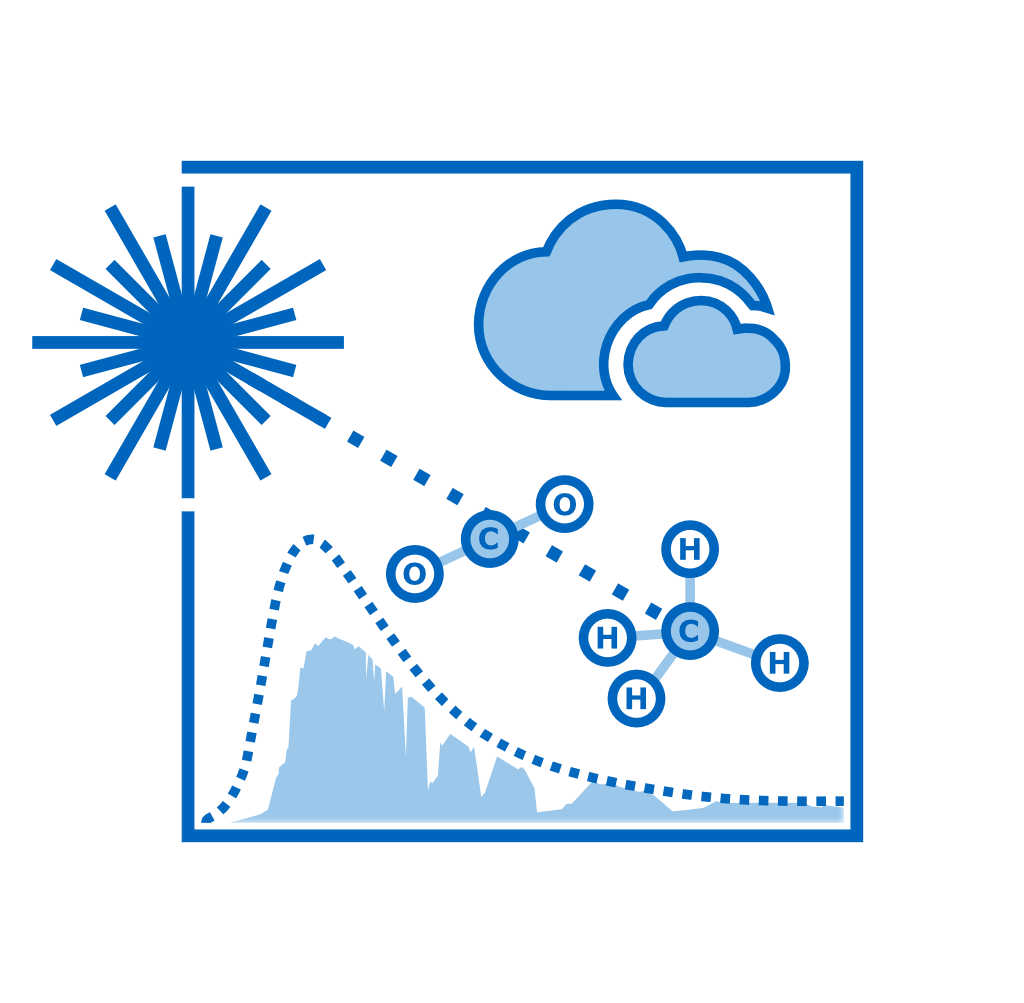
\includegraphics[height=20mm]{template/logos/esm-logo-square.png}
    }{}

\end{titlepage}

\thispagestyle{empty}
\vspace*{0.8\textheight}
\noindent
I confirm that this \MakeLowercase{\getDoctype{}} is my own work and I have documented all sources and material used.

\vspace{15mm}
\noindent
\getSubmissionLocation{}, \getSubmissionDate{} \hspace{50mm} \getAuthor{}

\cleardoublepage{}

\addcontentsline{toc}{chapter}{Acknowledgments}
\thispagestyle{empty}

\vspace*{20mm}

\begin{center}
    {\usekomafont{sectioning}\usekomafont{section} Acknowledgments}
\end{center}

\vspace{10mm}

Duis qui ea sint proident cillum sint sint culpa pariatur duis sunt commodo consequat reprehenderit. Officia sit veniam laborum aliqua. Minim reprehenderit consectetur laborum sint laboris quis et ullamco cillum adipisicing reprehenderit. Nostrud ullamco quis do ea cillum nostrud occaecat amet adipisicing aliqua aliquip.

\cleardoublepage{}

\chapter{\abstractname}

Global warming poses a significant challenge to our planet.
Emission Inventories have emerged as essential tools for climate mitigation.
However, they may be inaccurate, which motivates the need for inversion techniques that invert atmospheric transport using meteorological data and concentration measurements of greenhouse gases.
Typically, these inversion techniques require accurate priors.
Recent work has successfully investigated the applicability of compressed sensing in urban environments, alleviating the need for such priors.
This thesis builds on these approaches, investigating the applicability of compressed sensing techniques based on machine learning.
In particular, this thesis investigates an approach based on generative models.

A dataset of urban emission flux fields with a resolution of $1 \unit{km} \times 1 \unit{km}$ is built based on the high-resolution TNO-GHGco emission inventories from $2015$ and $2018$.
Three cities, Munich, Paris, and Zurich, are selected as case studies.
A variational autoencoder (VAE) is then trained on this dataset and evaluated on atmospheric inversion tasks, assuming that the largest emitters and background emissions are known. 

In particular, measurements are taken in simulated experiments with artificial footprints based on Gaussian plume simulations.
The reconstructions are evaluated based on relative error and SSIM and compared to a regularized least squares approach and sparse reconstruction algorithms using discrete cosine and discrete wavelet transforms.
Overall, the results show the competitive performance of the VAE with the approaches above for Munich and Zurich, while it fell short for Paris.
The VAE demonstrates a general strength in the structural similarity.

This thesis further experiments with modifications of the signal space the generator can generate, also called the range of the generator, by altering the latent dimension of the VAE and fine-tuning it to the case study cities.
These experiments reveal a trade-off between the size of the range and the search in that space, with a larger range decreasing the representational error; however, more information is required to find solutions.
The fine-tuned models improve the reconstruction performance significantly, beating the other approaches significantly for Munich and Zurich while closing the performance gap for Paris.
However, open work remains to investigate how these fine-tuned models deal with uncertainties in the inventories.

Finally, the generator is investigated in a controlled benchmark, revealing that this model does not fully capture the emission flux field distribution.
This limitation can likely be attributed to a need for more training data.

Overall, this thesis demonstrates that approaches based on machine learning are promising for urban emission flux reconstruction, with the potential for enhancement through more comprehensive urban datasets.


\clearpage

\glsnogroupskiptrue
\printnoidxglossaries

\clearpage

\microtypesetup{protrusion=false}
\tableofcontents{}
\microtypesetup{protrusion=true}

\mainmatter{}

% !TeX root = ../main.tex
% Add the above to each chapter to make compiling the PDF easier in some editors.

\chapter{Introduction}\label{chapter:introduction}

\begin{enumerate}
	\item Medical Imaging
	\item Global Warming
	\item Optional: Emission Inventories
	\item Area sources are not sparse and thus sparse reconstruction does not work well on them without transform
\end{enumerate}

\section{Motivation}
Bottom-up emission estimations are inaccurate.
Instead, top-down approaches could be used.
... et al. demonstrate that top-down approaches can be represented as an inverse problem with measurements $y$ and the emission field as $x$.
The transport of ghg molecules can be modeled as a linear map $A$ between $y$ and $x$, resulting in the following inverse problem:
\begin{equation}
	y = Ax
\end{equation}
In their paper, ... et al. show that using

Three reasons for bottom-up approach:
\begin{itemize}
	\item find unknown emitters
	\item determine diff. between bottom-up \& top-down
	\item find emitters not captured by inventories
\end{itemize}

\section{Research Questions}
This thesis aims at answering some questions:

\begin{itemize}
	\item How well can a variaional autoencoder capture a low dimensional representation of area sources in emission inventories?
	\item What is the effect of the dimension of that low dimensional space?
	\item Is the variational autoencoder generazible to all urban emission fields or should it be specialized on one city?
	\item How well does such a variational autoencoder perform in atmospheric inversion of area sources as a downstream task compared to state of the art approaches?
\end{itemize}

% !TeX root = ../main.tex
% Add the above to each chapter to make compiling the PDF easier in some editors.

\chapter{Related Work}\label{chapter:related_work}

\section{Compressed Sensing}
There are three main approaches to alleviate sparsity constraint.
1) transforms, such as Wavelet
2) only searching for unknown emissions and take esimtations as basis
3) Deep learning based approaches

\section{Deep Learning for Inverse Problems}
The field of medical imaging has made advancements in the inverse problems using deep learning.

\section{Generative Models}

\section{Contributions}

% !TeX root = ../main.tex
% Add the above to each chapter to make compiling the PDF easier in some editors.

\chapter{Dataset}\label{chapter:dataset}

This thesis aims to develop a compressed sensing framework that leverages the strengths of deep generative models.
Methods proposed by \textcite{CSUsingAI} have demonstrated superior reconstructions with fewer measurements than classical compressed sensing techniques.
Consequently, this thesis focuses on reconstructing ill-posed problems with many unknowns.

Datasets with high spatial resolution inventories are required to facilitate this.
Datasets like CAMS-REG-v4 \parencite{CAMS} provide \gls{GHG} emissions at a resolution of $0.1^{\circ}$ latitude by $0.05^{\circ}$ longitude, which corresponds to approximately $5$ by $5$ kilometers over central Europe.
This resolution is relatively low.
For example, a city spanning a $30 \unit{km}$ by $30 \unit{km}$ area would be divided into a spatial grid of $6$ by $6$ cells.
Therefore, this thesis utilizes the high-resolution inventories TNO-GHGco-v1.1 for $2015$ emissions \parencite{TNO_HighRes15} and TNO-GHGco-v4 for $2018$ emissions \parencite{TNO_HighRes18}.
These inventories provide emissions at spatial resolution of ${{}^{1}\!/\!{}_{120}}^\circ$ latitude by ${{}^{1}\!/\!{}_{60}}^\circ$ longitude, or approximately $1 \unit{km}$ by $1 \unit{km}$.
This high spatial resolution allows for extracting detailed emission fields in urban environments.
The inventories include \gls{GHG} emissions for each GNFR sector, with the road sector (sector F) further divided into four subsectors, for each coordinate in a defined European grid.
This results in $15$ emission values per gas per cell.

In this thesis, only $\text{CO}_2$ emissions from fossil fuels (ff) are considered.
However, the approaches presented can be directly applied to all \gls{GHG} sources.
Furthermore, as point sources are assumed to be known, only diffuse or area sources are extracted from the inventories.
Finally, it has to be noted that the following approximation is made: one grid cell has the spatial dimension of exactly $1 \unit{km}$ by $1 \unit{km}$.
While this may result in improper scaling of values for many cities, the final results remain unaffected due to the invariance of the inverse problem to scale.

\section{Urban Emission Fields}
Urban environments differ from non-urban environments in terms of their emissions.
For instance, urban environments often have a city center that generates a large portion of emissions, as can be seen in Munich in Figure \ref{fig:munich_emissions}.
\begin{figure}
    \centering
    \begin{subfigure}{0.32\textwidth}
        \centering
        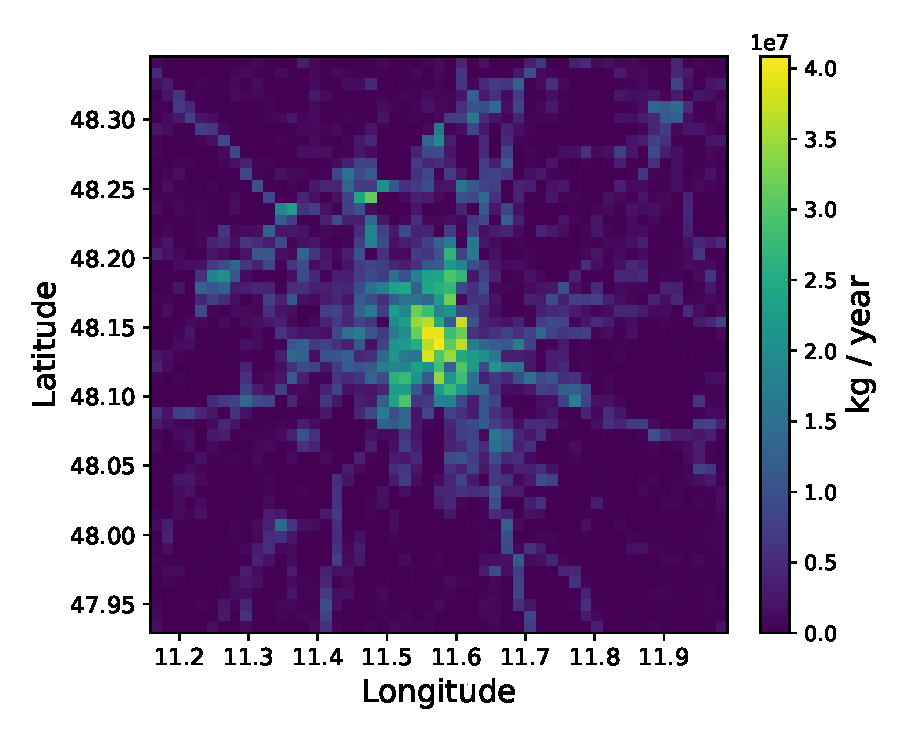
\includegraphics[width=\linewidth]{figures/03_dataset/munich/munich_2015_total_emissions.eps}
        \caption{Total Emission Fluxes}
    \end{subfigure}
    \begin{subfigure}{0.32\textwidth}
        \centering
        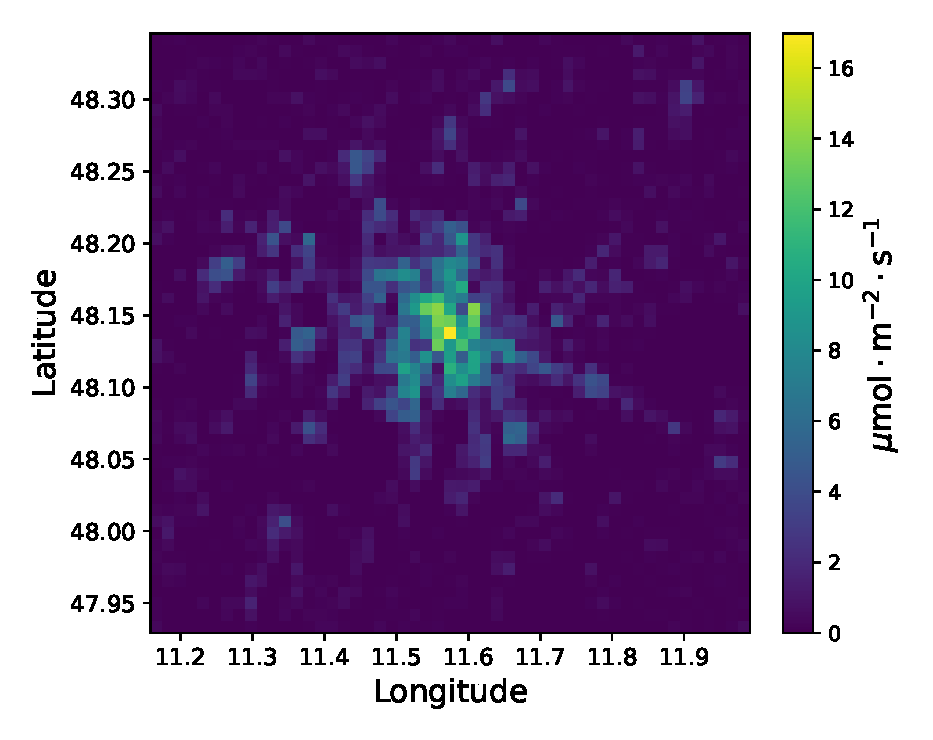
\includegraphics[width=\linewidth]{figures/03_dataset/munich/munich_2015_sector_c.eps}
        \caption{GNFR Sector C}
    \end{subfigure}
    \begin{subfigure}{0.32\textwidth}
        \centering
        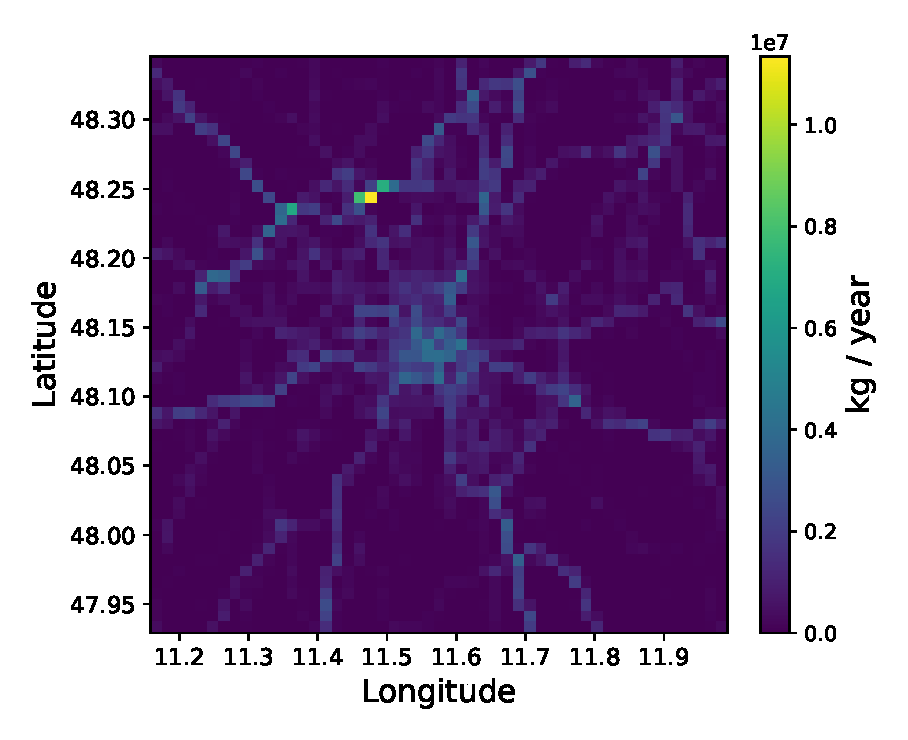
\includegraphics[width=\linewidth]{figures/03_dataset/munich/munich_2015_sector_f1.eps}
        \caption{GNFR Sector F1}
    \end{subfigure}
    \caption{$\text{CO}_2$ (ff) Emission Fluxes from Area Sources in Munich in 2015 \parencite{TNO_HighRes15}}
    \label{fig:munich_emissions}
\end{figure}
Therefore, as this thesis focuses on urban environments, they have to be filtered from the TNO-GHGco datasets.
For this, several cities are selected from a public database by OpenDatasoft \parencite{OpenDataSoft}.
Cities are filtered according to their population size.
For this thesis, we define a population threshold of $100,000$.
Any cities with a population greater than $100,000$ are selected for the dataset.

The coordinates of the filtered cities are then used to extract emission fields.
From the inventories, $51$ by $51$ grid cells around the city center are extracted.
This corresponds to a dimension of approximately $51 \unit{km}$ by $51 \unit{km}$. 
While most cities are not even close to this size, this allows for later cropping of the fields to a desired size.
For this thesis, emission fields have a final size of $32$ by $32$.

Some cities may be too close to each other, resulting in data leakage to test and validation sets.
Thus, cities are filtered if they are too close to other cities.
The following algorithm guarantees that no cities in the dataset overlap.

\begin{quotation}
First, an empty list of extracted lists is initialized.
Then, for each city, the latitude and longitude distances to all extracted cities are calculated.
In the next step, the algorithm determines which cities fall within a defined distance threshold from the current city.
If no cities are found within this threshold, the current city is added to the list, and the algorithm moves on to the next city.
However, if overlapping cities are identified within the threshold, the population size of the current city is compared to those of the overlapping cities.
If the current city has a larger population than all of the overlapping cities, these cities are removed, and the current city is added to the list.
If the current city does not have a larger population, it is ignored, and the algorithm continues with the next city.
\end{quotation}

This extraction results in $106$ city emission fields per year, $2015$, and $2018$.
However, we identified Bratislava as an outlier for this dataset due to its high \gls{SSIM} with a $0$ emission field.
Therefore, we exclude Bratislava from the dataset, thus reducing the number of cities to $105$.

This limited number of extracted emission fields is insufficient to train a generative model.
Thus, temporal scaling factors from \parencite{ScalingFactors} are useful for artificially generating more samples.
Scaling factors are applied to individual GNFR sectors.
This results in $24 \cdot 7 \cdot 12 = 2016$ samples per city per year.
The resulting combined dataset size is then $105 \cdot 2 \cdot 2016 = 423,360$ individual emission fields with size $51$ by $51$.
Scaling factors are applied at sampling time to reduce memory overhead, thus only keeping the original data in memory.

\section{Dataset Split}
The emission fields are divided into training, validation, and test sets.
The test set comprises $t$ percent of the data and is used exclusively for experiments and evaluations; the model does not encounter this data during training.
The validation set makes up $v$ percent of the data and is used during training to assess the model's generalization capabilities.
The remaining data, i.e., $1-v-t$ percent, is allocated to the training set for updating the model's weights.

A random split could result in unrepresentative subsets since emission fields of cities may vary significantly in their mean emissions.
For example, if the validation set contains cities with higher mean emissions, the \gls{MSE} during validation would be higher due to \gls{MSE}'s sensitivity to scale.
Therefore, it is essential to distribute cities equally across the training, validation, and test sets concerning their mean emissions to best assess generalization abilities.
Additionally, data from individual cities should not be split across different datasets to prevent data leakage.
For instance, Berlin's data from $2015$ should not be in the test set if its $2018$ data is in the training set.

The following algorithm fulfills both requirements from above while producing a reproducible split:

\begin{quotation}
First, the algorithm groups the emission fields according to their city name.
The emission fields are then sorted alphabetically according to the above names.
In the second step, the algorithm sorts the emission fields by their mean emissions in descending order.
Finally, it splits the dataset using equidistant indices to produce two datasets.
\end{quotation}

This algorithm is then used to assign $t$ percent of the data to the test set.
Then, from the remaining $1 - t$ percent, $\frac{v}{1 - t}$ percent is assigned to the validation set.
The rest is allocated to the training set.

\section{Data Augmentation}
To enhance the generalization capabilities of the model, we apply common image augmentation \parencite{ImageAugmentation} to the emission fields in the training dataset.
The augmentation methods applied include random cropping, flipping, and rotation.
To introduce variability in spatial positioning, emission fields are randomly cropped to a spatial dimension of $32$ by $32$.
Additionally, with a probability of $0.5$, the emission fields undergo horizontal or vertical flipping.
Similarly, with a probability of $0.5$, they are rotated by $90$ degrees.
These techniques result in eight possible transformations for each emission field, including the original unaltered version.

An example of this augmentation process is illustrated in Figure \ref{fig:nuernberg_emissions}.
The figure shows the original and transformed emission fields for the Nuremberg area sources, highlighting how the summed emissions are altered through the applied transformations.

\begin{figure}[h!]
    \centering
    \begin{subfigure}{0.4\textwidth}
        \centering
        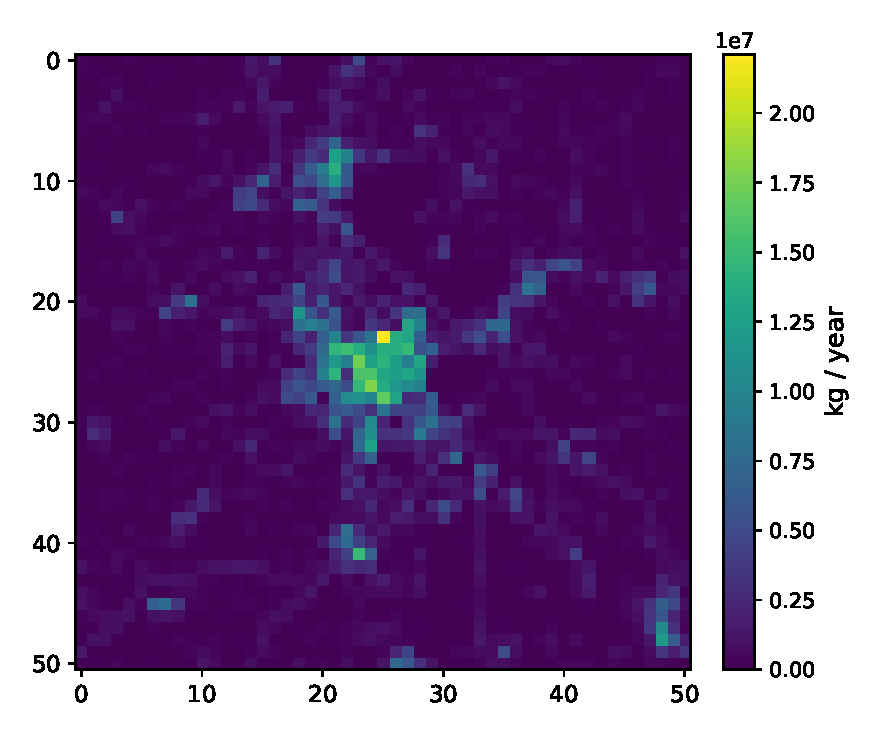
\includegraphics[width=\linewidth]{figures/03_dataset/nuernberg/nuernberg.eps}
        \caption{Original}
    \end{subfigure}
    \begin{subfigure}{0.4\textwidth}
        \centering
        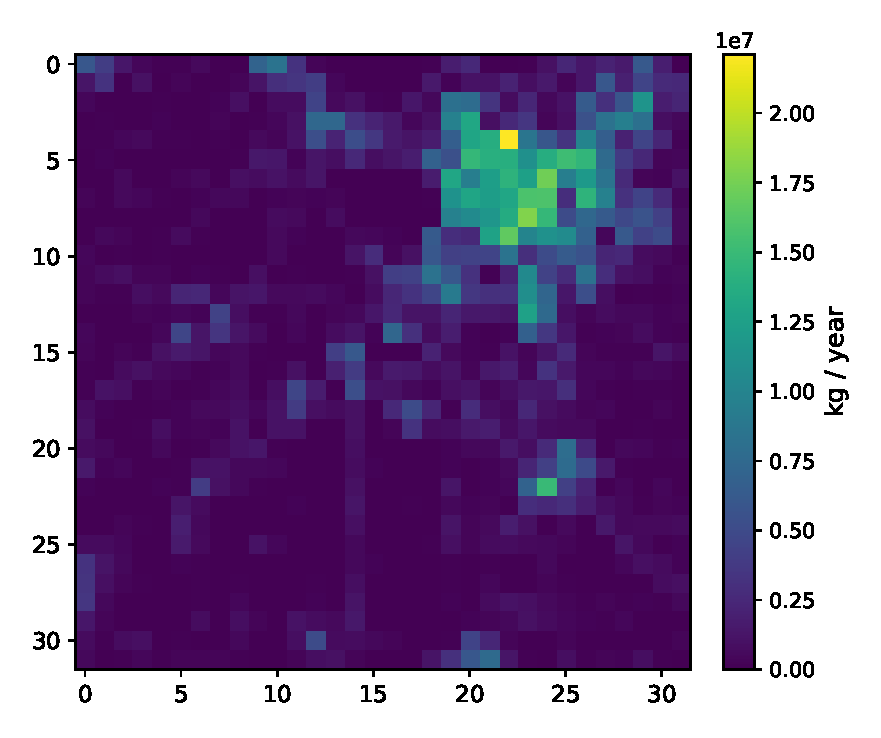
\includegraphics[width=\linewidth]{figures/03_dataset/nuernberg/nuernberg_transformed.eps}
        \caption{Transformed}
    \end{subfigure}
    \caption{Total $\text{CO}_2$ (ff) Emission Fluxes from Area Sources in Nuremberg in 2015 \parencite{TNO_HighRes15}}
    \label{fig:nuernberg_emissions}
\end{figure}

It is important to note that these transformations are not applied to the validation and test emission fields, except for a center crop to match the expected input dimensions.

\section{Scaling}
Scaling plays an important role in machine learning.
Large-scale data can make training converge slowly and become unstable \parencite{DataScaling}.
A common technique for scaling values is min-max scaling \parencite{MinMaxScaling}.
However, min-max scaling is sensitive to outliers and thus not ideal for emission inventories where the range of emissions within a city can vary greatly.
Instead, robust scaling can be applied.
To determine a good scaling factor, the $95$th percentile of values is determined for each city in the training set.
The inverse of the average is then used as the scaling factor.
The resulting scaling factor is thus $\frac{1}{2.5 * 10^6}$ after rounding.
All experiments are, without loss of generality, performed on the scaled data.

\section{Case Studies}
In addition to the test data used for model performance evaluation, three cities are selected for detailed case studies.
The cities are Munich, Zurich, and Paris.
These cities are chosen based on the ICOS Cities PAUL project \parencite{Icos} and represent a range of city sizes, from small to medium and large.
In order to ensure unbiased results, these cities are excluded from the dataset prior to splitting, reducing the total number of cities available for training from $105$ to $102$.
These cities allow closer inspection of the outputs of different algorithms.

% !TeX root = ../main.tex
% Add the above to each chapter to make compiling the PDF easier in some editors.

\chapter{Variational Autoencoder}\label{chapter:vae}

Some text about generative models and variational autoencoder \parencite{VAE} in its original form being the chosen one.

\section{Architecture Search}
Searching for optimal hyperparamaters is a challenging task with many different approaches \parencite{HyperParameters}.
In particular, designing a good architecture takes a lot of trial and error.
Thus, different architectures are explored to determine a suitable one.
For this, first a basline architecture is established.
Then, different variations of this architecture are explored and trained.
The architecture of the model with the best performance is then chosen as the model architecture for this thesis.

Each variation is trained with for $20$ epochs on the TNO 2015 data only to decrease the architecture bias during search.
The dataset split is $t=0.15$, $v=0.15$, with the test set not being used at all.
The batch size is $32$.
As optimizer AmsGrad \parencite{AmsGrad} is used with a learning rate of $\dots$.
Gradients are clipped at $0.5$.
% Add any further hyperparameters.

\section{Baseline Architecture}
The baseline architecture is inspired by \parencite{Tightrope}.
This means that the bottleneckl layers have a high width and height.
As the input width and height of the emission fields are $32$ by $32$, the Bottleneck width and height are chosen as $8$ by $8$.
Inspired by \parencite{AllConvolutional} , to reduce the width and height dimensions, instead of using pooling operations, $2$ strided convolutions are used.
The strided convolutions, depicted in Figure, have kernel 2 and stride 2, thus halfing the size.

\begin{figure}[h!]
    \centering
    \begin{minipage}[b]{0.45\textwidth}
        \centering
        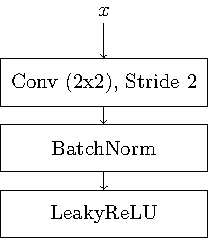
\includegraphics[]{figures/model_architecture/build/conv_layer.pdf}
        \caption{Conv Layer}
    \end{minipage}
    \hfill
    \begin{minipage}[b]{0.45\textwidth}
        \centering
        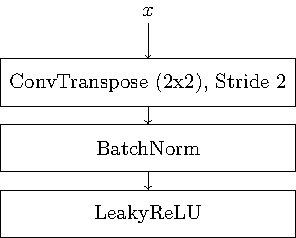
\includegraphics[]{figures/model_architecture/build/deconv_layer.pdf}
        \caption{DeConv Layer}
    \end{minipage}
\end{figure}

The strided convolution layers make use of the LeakyReLu activation function and batch normalization \parencite{BatchNorm}, as a regularization technique.

Vice versa, in the decoder, 2 strided transpose convolutions with the same parameters are used to double the width and height instead of upsampling layers.

In between the strided convolutions residual convolutional layers (ResConv) \parencite{ResNet} are used.
They can be seen in Figure.
\begin{figure}[h!]
    \centering
    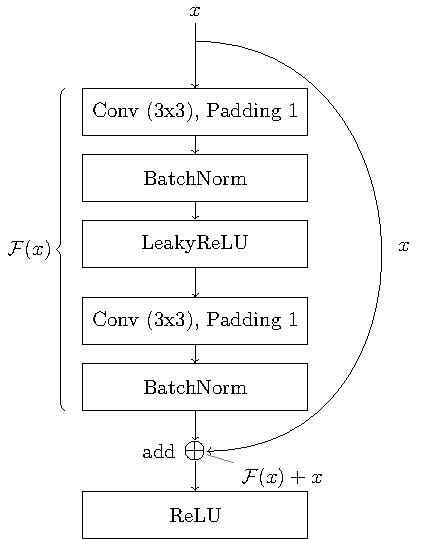
\includegraphics[]{figures/model_architecture/build/residual_conv_layer.pdf}
    \caption{ResConv Layer \parencite{ResNet}}
\end{figure}
The ResConv layers make use of two convolutions with kernel 3 and padding 1 to retain the width and height dimensions.
The output activation is ReLu.
In between the two convolutional layers, LeakyReLu is used again.
Again, batchnorm is applied.
\begin{figure}[h!]
    \centering
    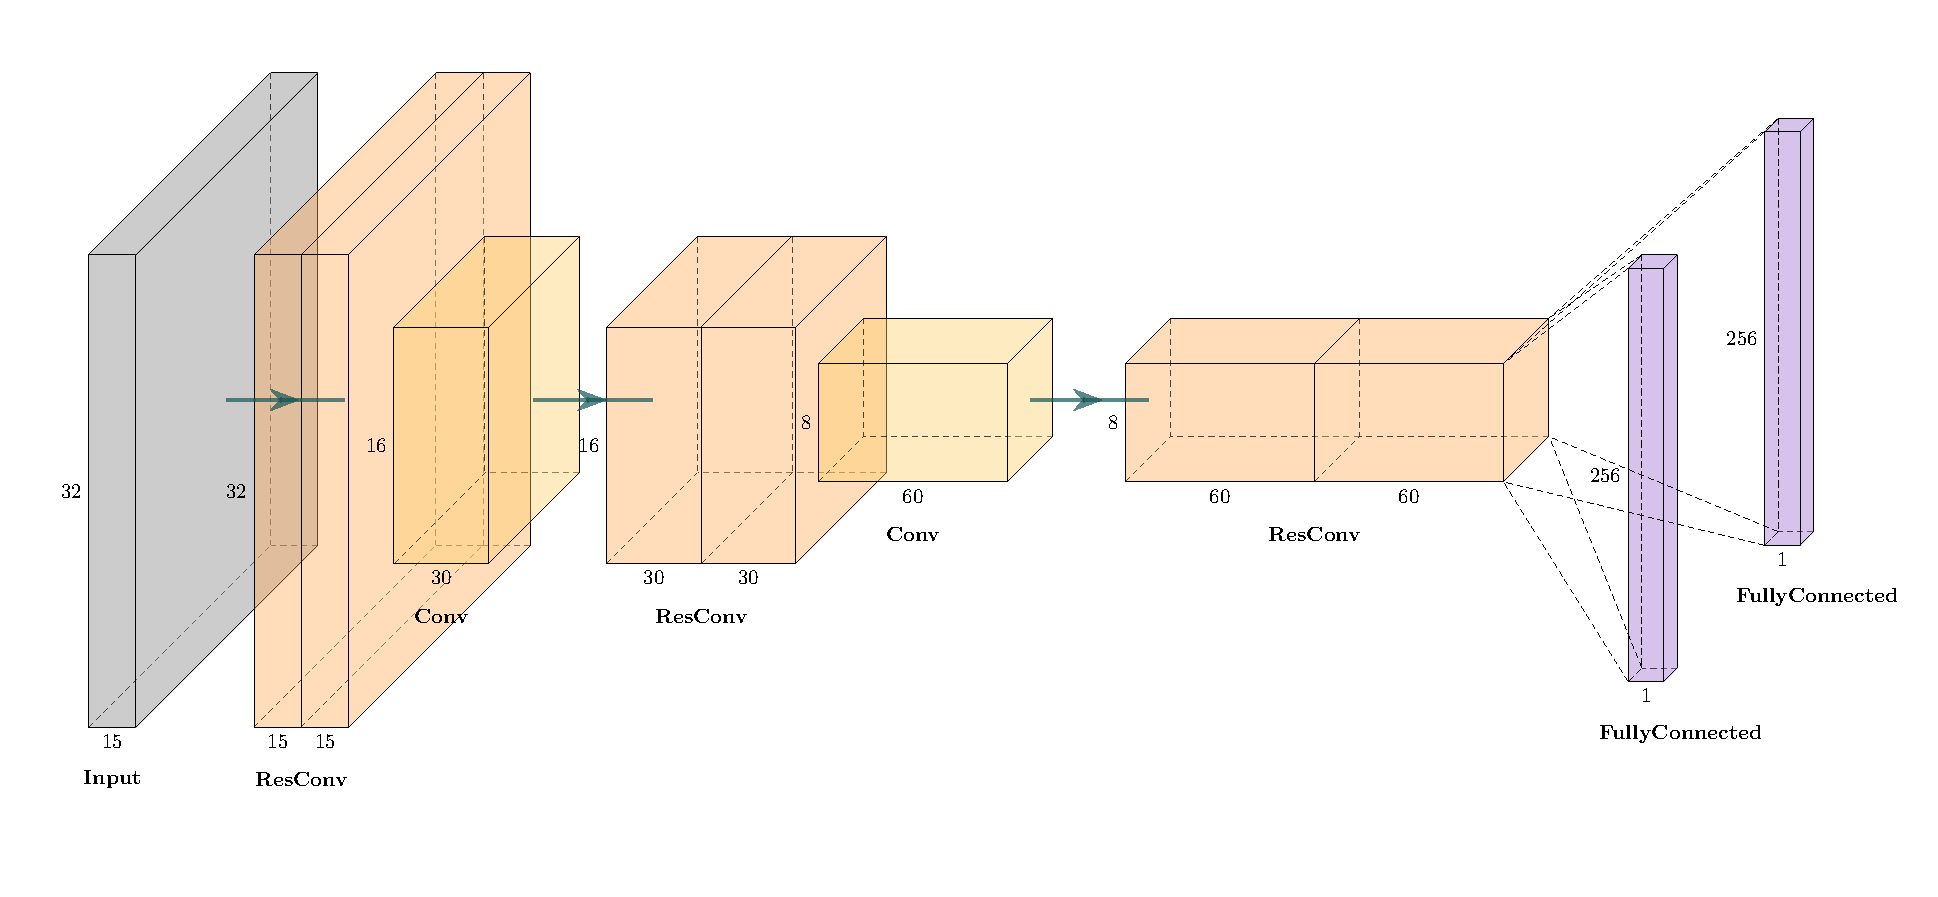
\includegraphics[width=\textwidth]{figures/model_architecture/build/baseline_vae_encoder.pdf}
    \caption{Baseline Encoder Architecture (generated with \parencite{NNVisualization})}
\end{figure}
\begin{figure}[h!]
    \centering
    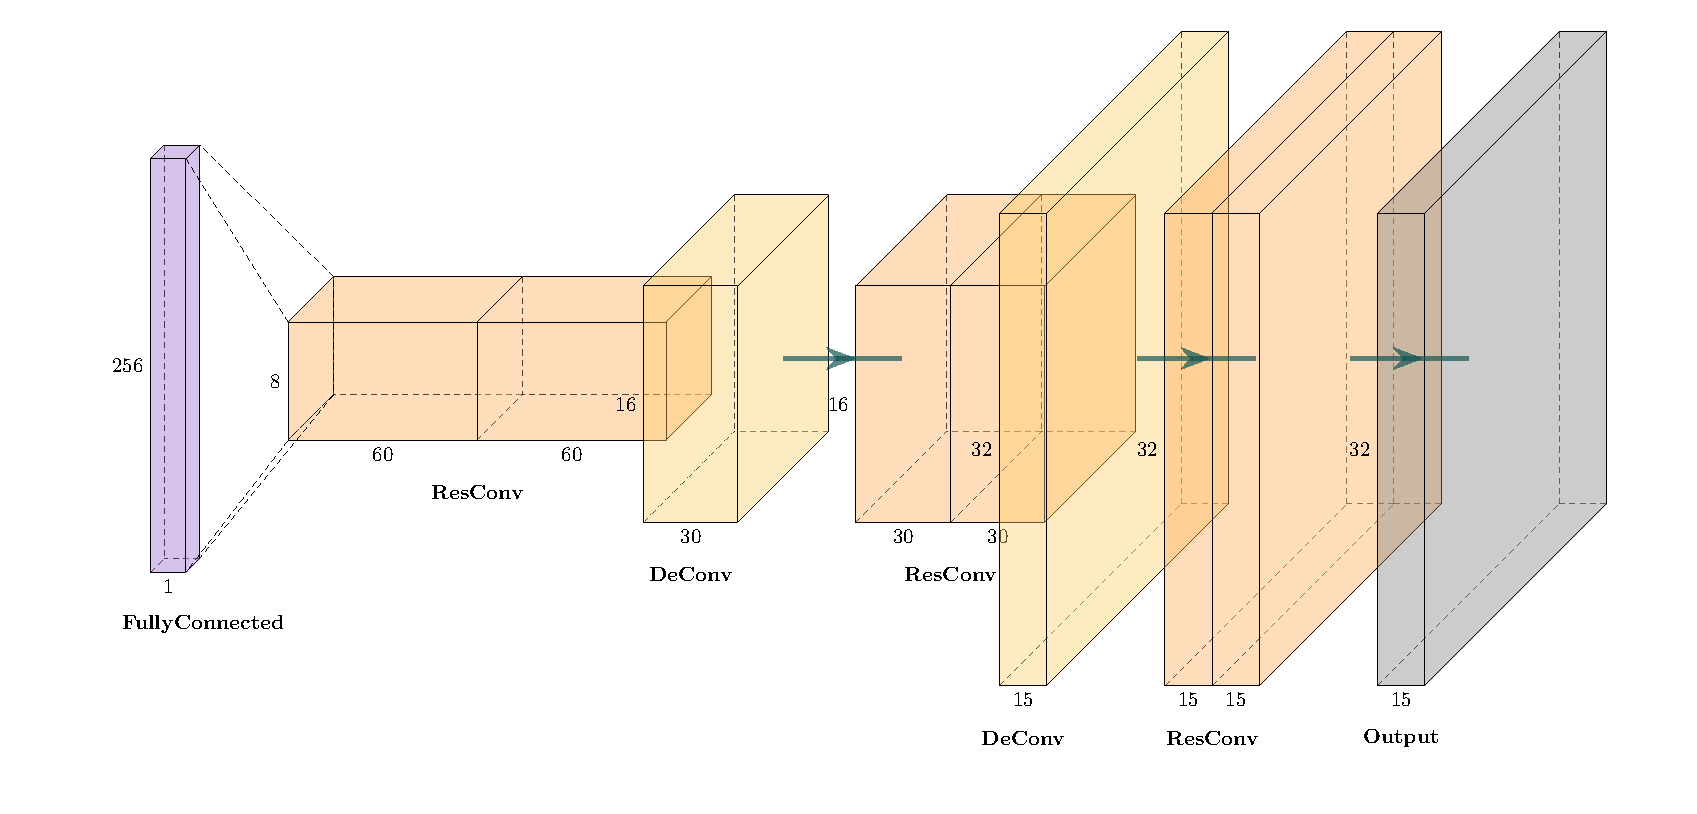
\includegraphics[width=\textwidth]{figures/model_architecture/build/baseline_vae_decoder.pdf}
    \caption{Baseline Decoder Architecture (generated with \parencite{NNVisualization})}
\end{figure}
As can be seen in Figure and Figure, the 2 strided convolutions are located between $2$ layers of ResConv layers each, in the encoder and decoder.
Fully connected layers are used at the end of the encoder and beginning of the decoder to achive a hidden dimension $256$ of the latent space. 
The last ResConv layers does not use batch normalization.
The number of parameters is \dots.

The loss function used is the typical VAE loss with MSE loss as recontruction loss and Elbo \parencite{VAE} \dots .
\begin{equation}
    L(x, \hat{x}) = 1 + 2
\end{equation}
In addition to the loss, at each step the SSIM \parencite{SSIM} is computed as it provides qualitatively better comparison between two emission fields than the MSE as it takes structure into account.

\section{Explored Variations}
The following variations are explored
\begin{enumerate}
    \item conv layers to increase / decrease depth and pooling layers to decrease width/height and upsample layers to increase width/height
    \item upsampling emission fields to $64$ by $64$ and then applying convlutions; in decoder max pooling to downsample $64$ by $64$ to $32$ by $32$
    \item more depth; instead of doubling depth, quadrupling it
    \item 2 conv layers for changing width and height instead of one strided convolution
    \item 3 ResConv layers everywhere
    \item residual layers with identity mappings depicted in Figure based on \parencite{IdentityMappings} instead of ResConv layers from Figure
    \item residual layers with identity mappings with dropout \parencite{Dropout} based on \parencite{WideResNet} (add explanation)
\end{enumerate}

\begin{figure}[h!]
    \centering
    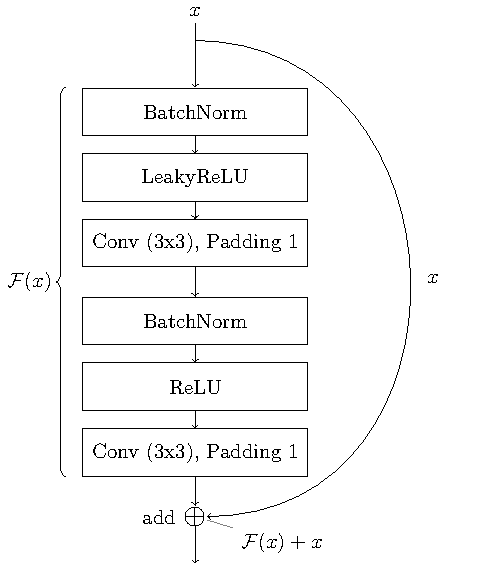
\includegraphics[]{figures/model_architecture/build/residual_conv_with_im_layer.pdf}
    \caption{ResConv Layer With Identity Mappings \parencite{IdentityMappings}}
\end{figure}

In Figure , the validation losses and validation SSIM can be seen from the 20 epoch trianing runs.

\begin{figure}
    \centering
    \begin{subfigure}{0.49\textwidth}
        \centering
        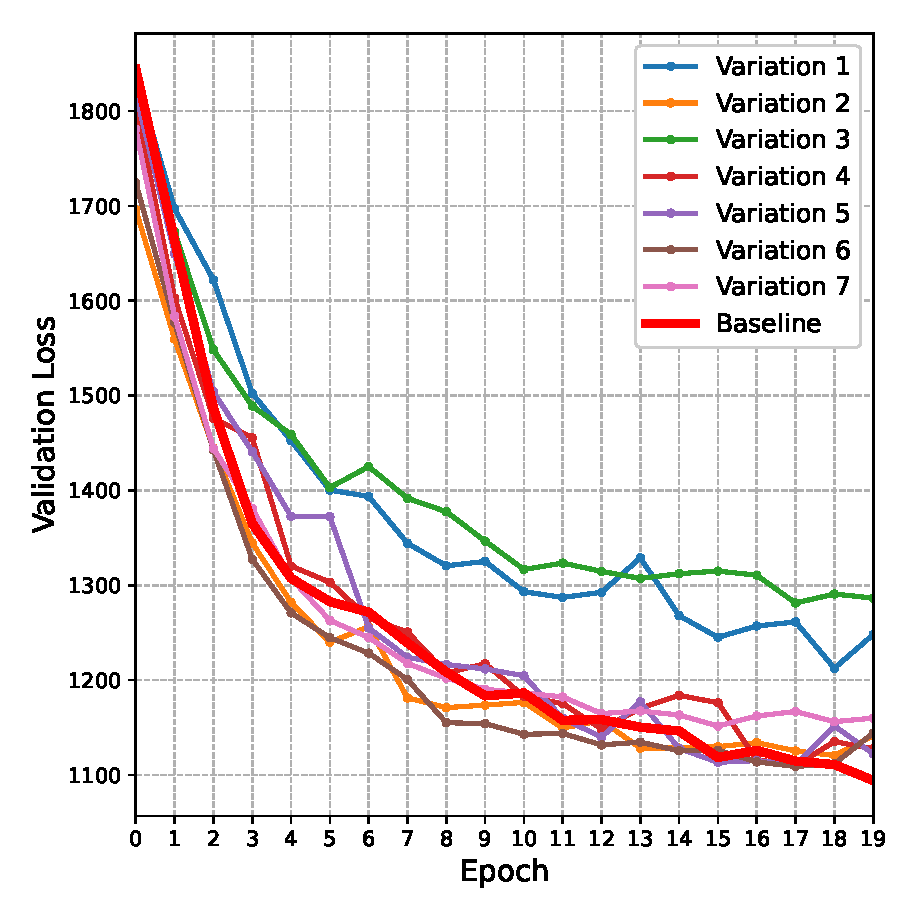
\includegraphics[width=\linewidth]{figures/architecture_search/architecture_search_loss.eps}
        \caption{Validation Loss}
        \label{fig:sub1}
    \end{subfigure}%
    \begin{subfigure}{0.49\textwidth}
        \centering
        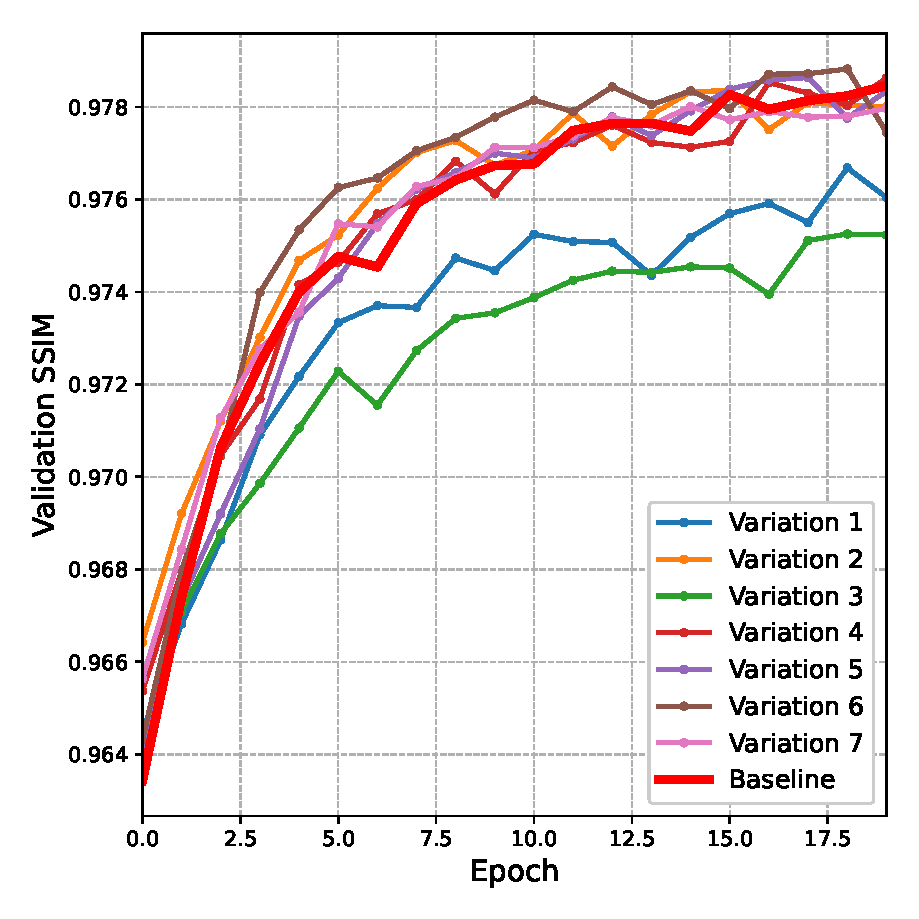
\includegraphics[width=\linewidth]{figures/architecture_search/architecture_search_ssim.eps}
        \caption{Validation SSIM}
        \label{fig:sub2}
    \end{subfigure}
    \caption{Performance of Variations on Validation Data During Training}
    \label{fig:test}
\end{figure}

Add some observations.

\section{Final Architecture}
From the previous subsection, it can be concluded that the baseline architecture performs very well.
The following changes are made to result in the final architecture.
First, the residual layers in Figure  with identity mappings are used.
Furthermore, they are extended with dropout as proposed in \parencite{WideResNet} in the \dots.
Finally, the number of residual layers are increased to $3$.
The encoder and decoder respectively can be seen in Figure and Figure.
\begin{figure}[h!]
    \centering
    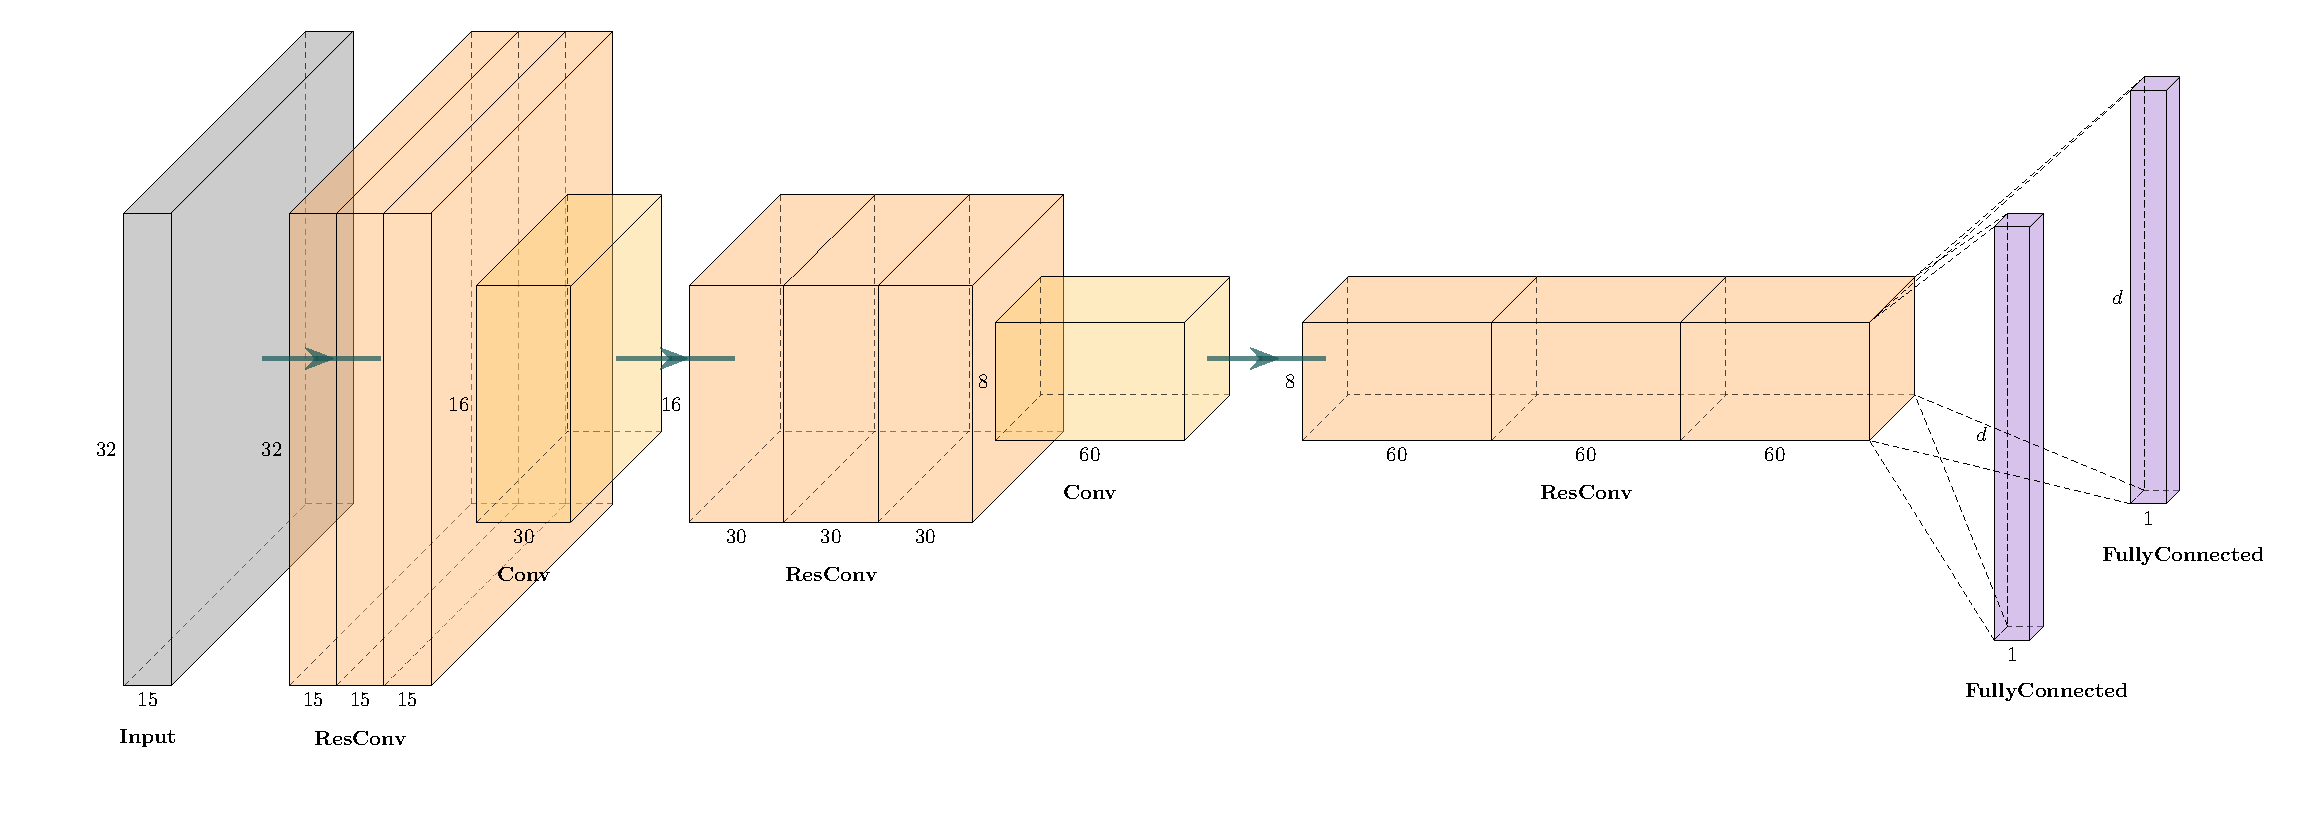
\includegraphics[width=\textwidth]{figures/model_architecture/build/final_vae_encoder.pdf}
    \caption{Final Encoder Architecture (generated with \parencite{NNVisualization})}
\end{figure}
\begin{figure}[h!]
    \centering
    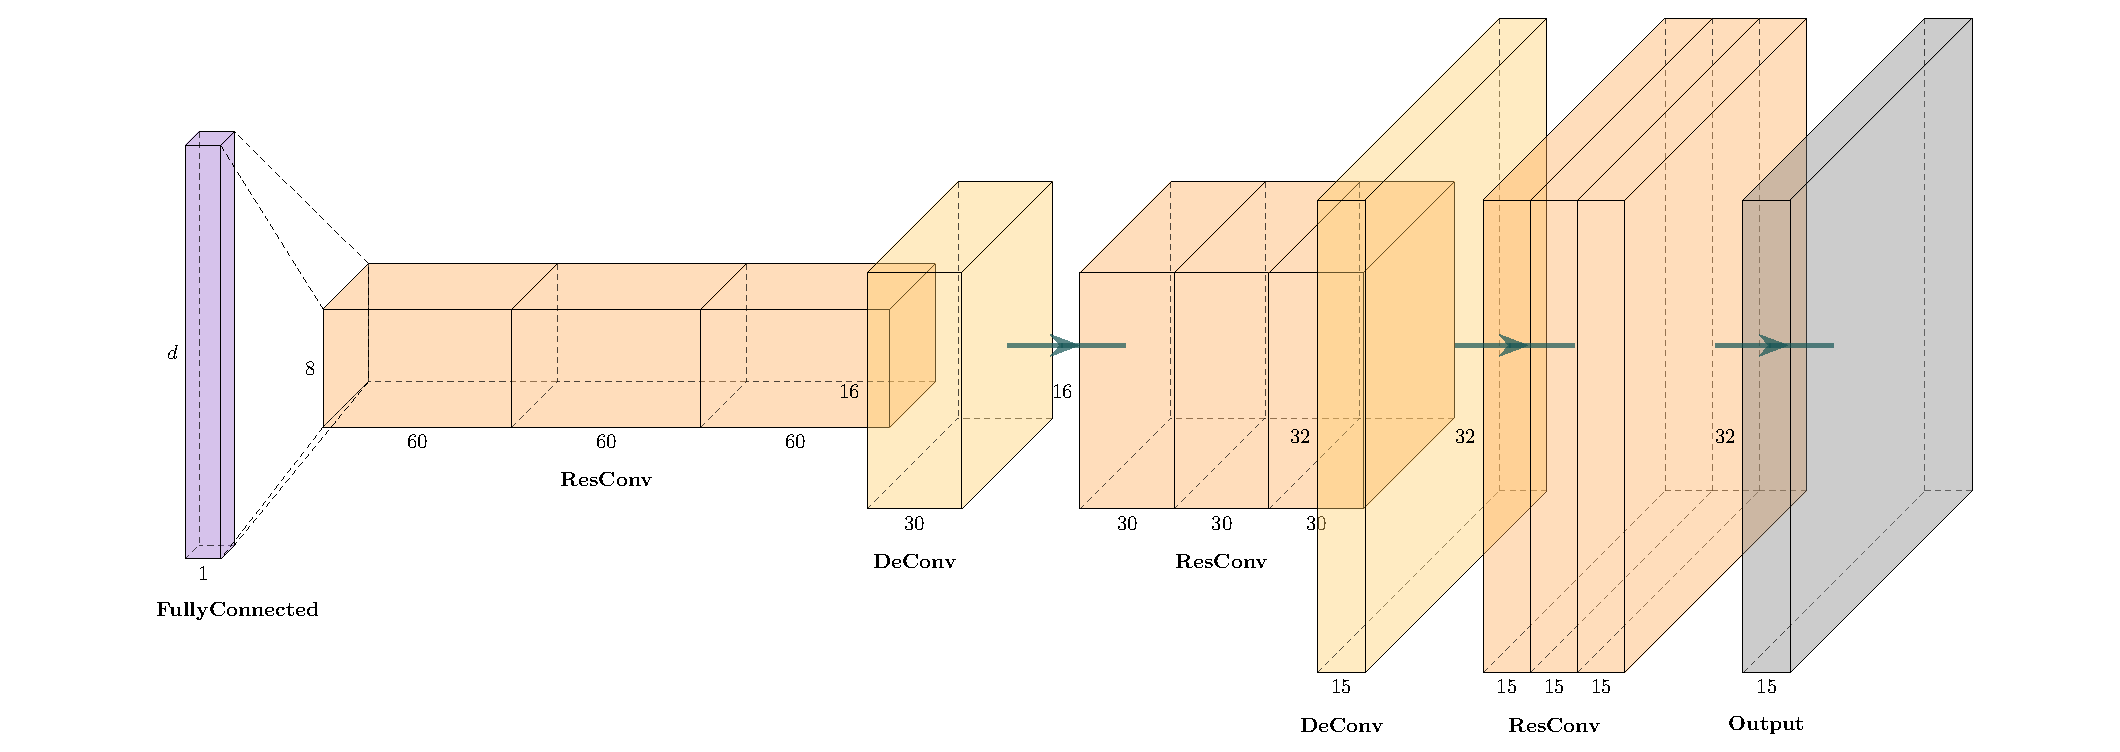
\includegraphics[width=\textwidth]{figures/model_architecture/build/final_vae_decoder.pdf}
    \caption{Final Decoder Architecture (generated with \parencite{NNVisualization})}
\end{figure}
The latent dimension $d$ which was kept at $d = 256$ for the "ablation study" is now kept parametrizable.
In fact, for this thesis, different latent dimensions are explored: $d \in \{ 256, 512, 1024, 2048 \}$.
The number of parameters of the model in dependence of $d$ are \dots.

\begin{table}[h]
    \centering
    \begin{tabular}{|c|c|c|}
        \hline
        \textbf{$d$} & \textbf{Encoder Parameters} & \textbf{Decoder Parameters} \\
        \hline
        \hline
        $256$ & 2.2 M & 1.3 M \\
        $512$ & 4.2 M & 2.2 M \\
        $1024$ & 8.1 M & 4.2 M \\
        $2048$ & 16.0 M & 8.1 M \\
        \hline
    \end{tabular}
    \caption{Number of Encoder / Decoder Parameters in Dependence of Latent Dimension $d$}
    \label{tab:num_parameters}
\end{table}

The models are trained on both the TNO 2015 and 2018 data for $100$ epochs.
The dataset split is $t = 0.13$ and $v = 0.15$, resulting in $13$ cities in the test, $15$ cities in the validation, and $74$ cities in the training set.
The exact split can be seen in appendix \dots.
The weights of the model with the highest validation SSIM during the $100$ epochs is stored.
All other relevant hyperparamaters are kept the same as in the the variations subsection.

The training losses, SSIM, and mean MSE can be seen in Figure for each $d$.
(add Figure).
It can be observed that there is overfitting present in the data.
This may be related to samples like London or Berlin in the trianing data that steer the loss, resulting in overfitting to these cities, due to their size of emissions.
The amount of overfitting decreases with an increase in $d$.


\section{Fine-tuning}
Fine-tuning is a popular technique to steer a model to do somthing more specific \cite{FineTuning}.
In the case of this thesis, fine-tuning the trained model to specific cities may make sense to achieve more precise recontruction.
The idea is that a generative model can learn the structure of the city and focus on differences of emissions due to observed data.
Thus, fine-tuning is evaluated in this thesis.
For this, the three for the case studies chosen cities are used.

The idea of fine-tuning the model to specific cities is to move the range $R(G)$ of the generator $G$, i.e. the space of all emission fields generateable by the decoder of the VAE.
For instance, if a model cannot represent an emission field that is to be sensed, it is not able to reconstruct the emission field due to a high representational error.
By fine-tuning the model, the range of the generator is modified such that the emission field to be sensed may either be closer to the range of the generator or even in it.
This is depicted in Figure (make figure here to show the idea).

During fine-tuning, the weights of the original models are updated.
The learning rate is reduced.
In our case, we chose $10^{-x}$ as learning rate.

For fine-tuning, the TNO 2015 data is used.
Later, for evaluation the TNO 2018 is used.

The cities are cropped in the center.
Furthermore, random scaling factors $s \in U(0.5, 1.5)$ are applied to simulate uncertainties in emission inventories.
Additionally, gaussian noise is added to the city emission field.

Models are fine-tuned for $30$ epochs which results in errors close to convergence.


% !TeX root = ../main.tex
% Add the above to each chapter to make compiling the PDF easier in some editors.

\chapter{Compressed Sensing}\label{chapter:compressed_sensing}

\section{Inverse Problems}

\subsection{Gaussian Measurements}
In order to evaluate the generative capbailities in the context of inverse problems, a compressed sensing problem is used for evaluation.
This compressed sensing problem is based on the paper by Bora et al. as they mention that the performance of generative models can be assesed based on their provided problem statement.
For this, a identically independent distributed matrix $A \in R^{m \times 15000}$ is sampled for each run.
The following inverse problem is then solved using the minimization problem proposed by Bora et al \parencite{CSUsingAI}.
\begin{equation}
    y = A x + \epsilon
\end{equation}
with $x$ being the emission fields $x^*$ in vectorized form.
This inverse problem is equivalnt to taking taking $m$ measurements that is randomly linearly affected by any sector in any cell within the emission field grid.
While this does not correspond to a typical transport model which follows the law of physics, this problem serves as a good proxy for evaluating the generative capbailities in the context of inverse problems of the trained VAE. 

The evaluation is performed on scaled emission fields.

The resulting pipeline is the following:
\begin{enumerate}
    \item Generate random A
    \item Sample x from test set
    \item Vectorize x
    \item Compute y from forward model
    \item Run reconstruction algorithm (minimization problem)
    \item Unvectorize resulting x dach
    \item Compare x with x dach
\end{enumerate}

The reconstruction algorithm is run for the following number of measurements:
For each of the numbers, the reconstruction is run for each emission field in the test dataset.
A random measurement matrix $A$ is generated and each of the $3$ algorithms solve the same inverse problem.
The temporal transforms are disabled during evaluation which means that for each city only one emission field per year is used.
The evaluation is run 5 times to reduce randomness resulting from random initialization of $z$.

\subsection{Gaussian Plume Model}
Gaussian sensing matrix do not represent the real the emission problem well.
Instead of randomly samples sensing matrices, transport models should be used that indicate the sensitivity of measurements with resepect to physical grid cells based on the transport of molecules in the past.
These transport models are computationally expensive to compute and in generel difficult to estimate on a per city basis.
Thus, we apply the same idea as Benji in his work.
We substitue typical transport models, such as STILT, with a Gaussian plume model.
In his paper, Benji reconstructed the emission field without considering the indivudal sectors as contributors.
In this thesis, a full reconstruction is attempted, i.e. all $15$ sectors are reconstructed.
Therefore, the sensing matrix based on the Gaussian plume model must be adapted accordingly.

The forward model is the following:
\begin{equation}
    y = [A, \dots, A] [x_{s_0}, \dots, x_{s_{14}}]^T
\end{equation}
$A$ is the Gaussian plume model for n measurements.
$x_{s_i}$ is the emission field for a single sector.

\section{Inverse Problem Solvers}

\subsection{Generative Model Solver}
Let $D: R^d \rightarrow R^{32 \times 32 \times 15}$ be the decoder of the variational autoencoder.
Then, the generator $G: R^d \rightarrow R^{15000}$ can be written as $G(z) = \text{vec}(D(z))$, i.e. the generator G is the vectorization of the decoder of the VAE.

The minimization problem
\begin{equation}
    z^* = \arg\min_{z}{\norm{A G(z) - y} + R(z)}
\end{equation}
with regularization term $R(z) = \norm{z}$ is solved numerically using the Adam Optimizer \parencite{Adam}.
For the learning rate, values are chosen based on the number of measurements, as seen in table (make table).
These values are determined empirically.

\subsection{LASSO}
To assess the capabilities of the generative model against other approaches, the sparse reconstruction algorithm using the LASSO objective is used.
\begin{equation}
    LASSO = 
\end{equation}
Scaling factor $\alpha$ is chosen as $0.1$, like in Bora et als paper.
In addition to the LASSO in the original basis, the problems is transformed into two further bases.
The first transform used for this is the discrete cosine transform.
The cosine coefficients are computed
The second transform is the discrete wavelet transform.
Wavelet coefficients are computed using \parencite{PyWavelets}.
Transformations are applied per sector.

% !TeX root = ../main.tex
% Add the above to each chapter to make compiling the PDF easier in some editors.

\chapter{Results}\label{chapter:results}
\section{Variational Auto Encoder Benchmark}
In this chapter, the following experiments are performed.
For all experiments the test data is used.
Then, an inverse problem is generated.
This is run x times.

\subsection{Latent Dimension}
The latent dimension of the VAE has an effect of the representational error.
With an increase of the latent dimension, the VAE is able to represent more information.
This means the range of the generator is bigger.
The representational error, i.e. the error observed if the complete field is sensed, is smaller.
However, with a bigger range, the search for a point becomes more difficult.
This results in the following [to fill].
\begin{figure}[h!]
    \centering
    \begin{subfigure}[b]{0.49\textwidth}
        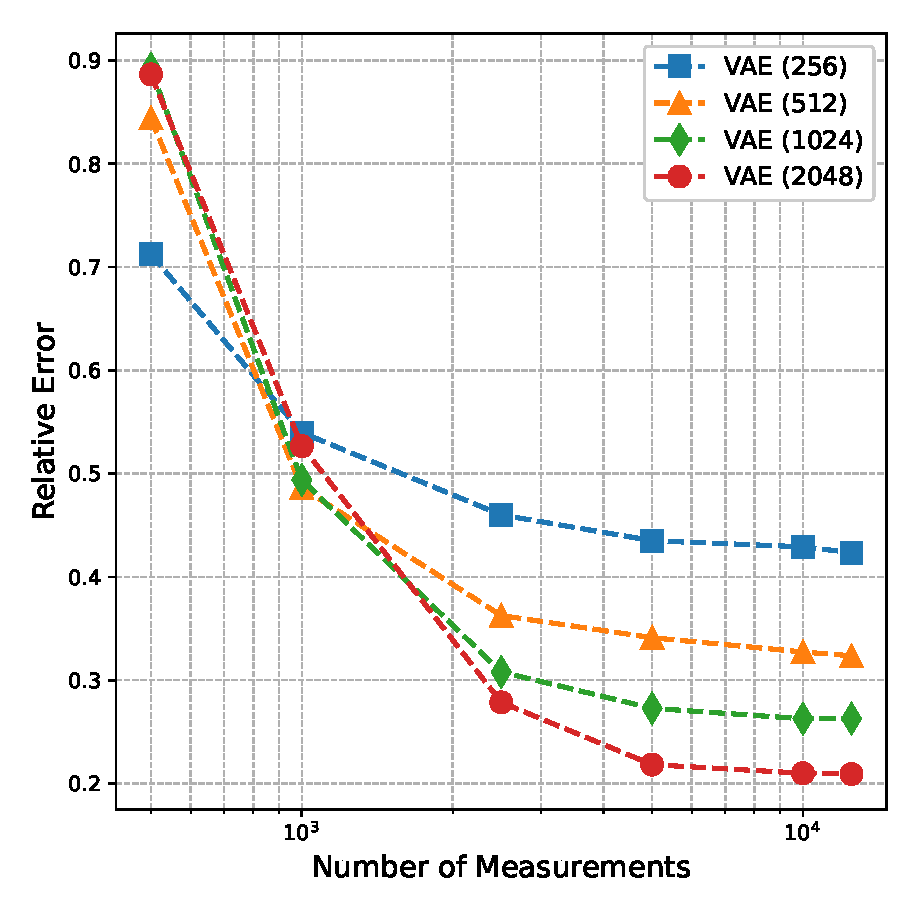
\includegraphics[width=\textwidth]{figures/06_results/vae_benchmark/effect_of_latent_dimension/effect_of_latent_dimension_relative_error.eps}
        \caption{Relative Error}
    \end{subfigure}
    \begin{subfigure}[b]{0.49\textwidth}
        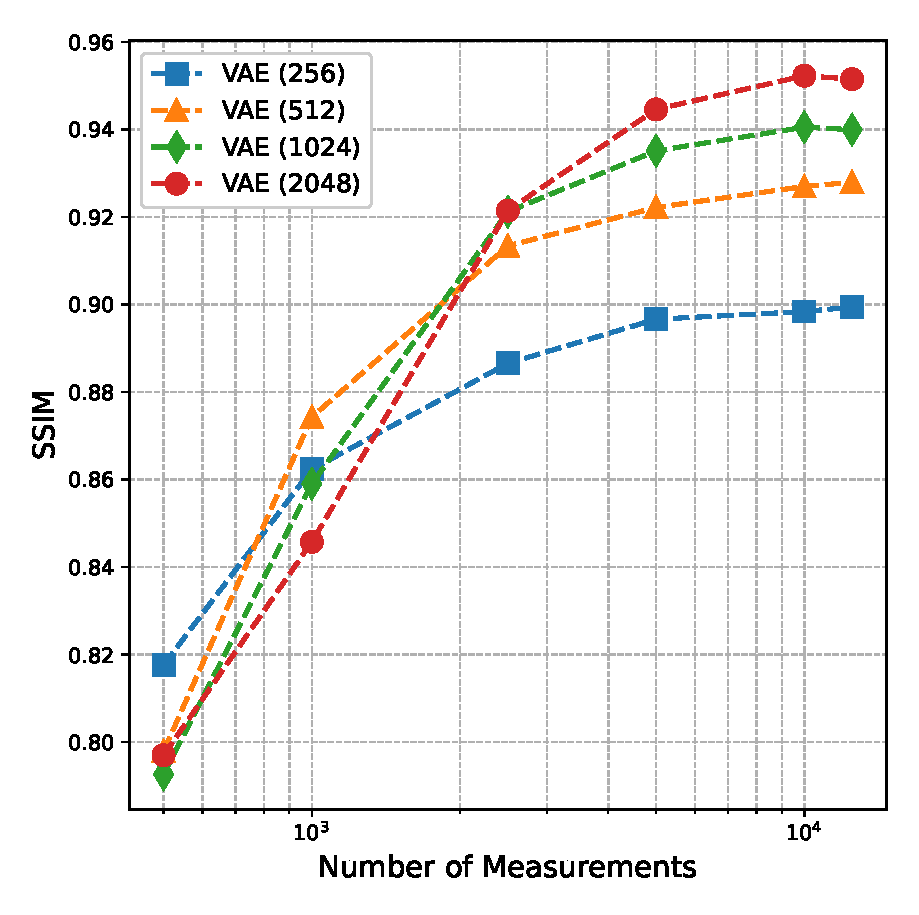
\includegraphics[width=\textwidth]{figures/06_results/vae_benchmark/effect_of_latent_dimension/effect_of_latent_dimension_ssim.eps}
        \caption{SSIM}
    \end{subfigure}
    \caption{Effect of Latent Dimension}
\end{figure}
A smaller latent dimension will have a smaller error for few measurements
A bigger latent dimension will have a smaller error for many measurements.

\subsection{Fine-tuned Models vs Base Models}

\begin{table}[h!]
    \centering
    \begin{tabular}{|c|c|c|c|c|}
        \hline
        \multirow{2}{*}{} & \multirow{2}*{\begin{tabular}{c}\textbf{Latent}\\\textbf{Dimension}\end{tabular}} & \multicolumn{3}{c|}{\textbf{City}} \\
        \cline{3-5}
        & & \textbf{Munich} & \textbf{Paris} & \textbf{Zurich} \\
        \hline
        \multirow{4}*{\begin{tabular}{c}\textbf{Relative Error}\\\textbf{Improvement}\end{tabular}}
            & 256 & \textbf{+30.87\%} & \textbf{+29.83\%} & \textbf{+31.32\%} \\
            & 512 & \textbf{+30.60\%} & \textbf{+31.59\%} & \textbf{+33.39\%} \\
            & 1024 & \textbf{+24.55\%} & \textbf{+20.20\%} & \textbf{+25.73\%} \\
            & 2048 & \textbf{+14.66\%} & \textbf{+14.54\%} & \textbf{+21.73\%} \\
        \hline
        \multirow{4}{*}{\begin{tabular}{c}\textbf{SSIM}\\\textbf{Improvement}\end{tabular}}
            & 256 & \textbf{+0.02\%} & \textbf{+5.43\%} & -4.14\% \\
            & 512 & -2.54\% & \textbf{+5.71\%} & -3.69\% \\
            & 1024 & -1.67\% & \textbf{+4.03\%} & -4.61\% \\
            & 2048 & -1.63\% & \textbf{+2.10\%} & -4.53\% \\
        \hline
    \end{tabular}
    \caption{Relative Error and SSIM Improvements from Fine-tuning}
    \label{tab:results}
\end{table}


% \begin{figure}[h!]
%     \centering
%     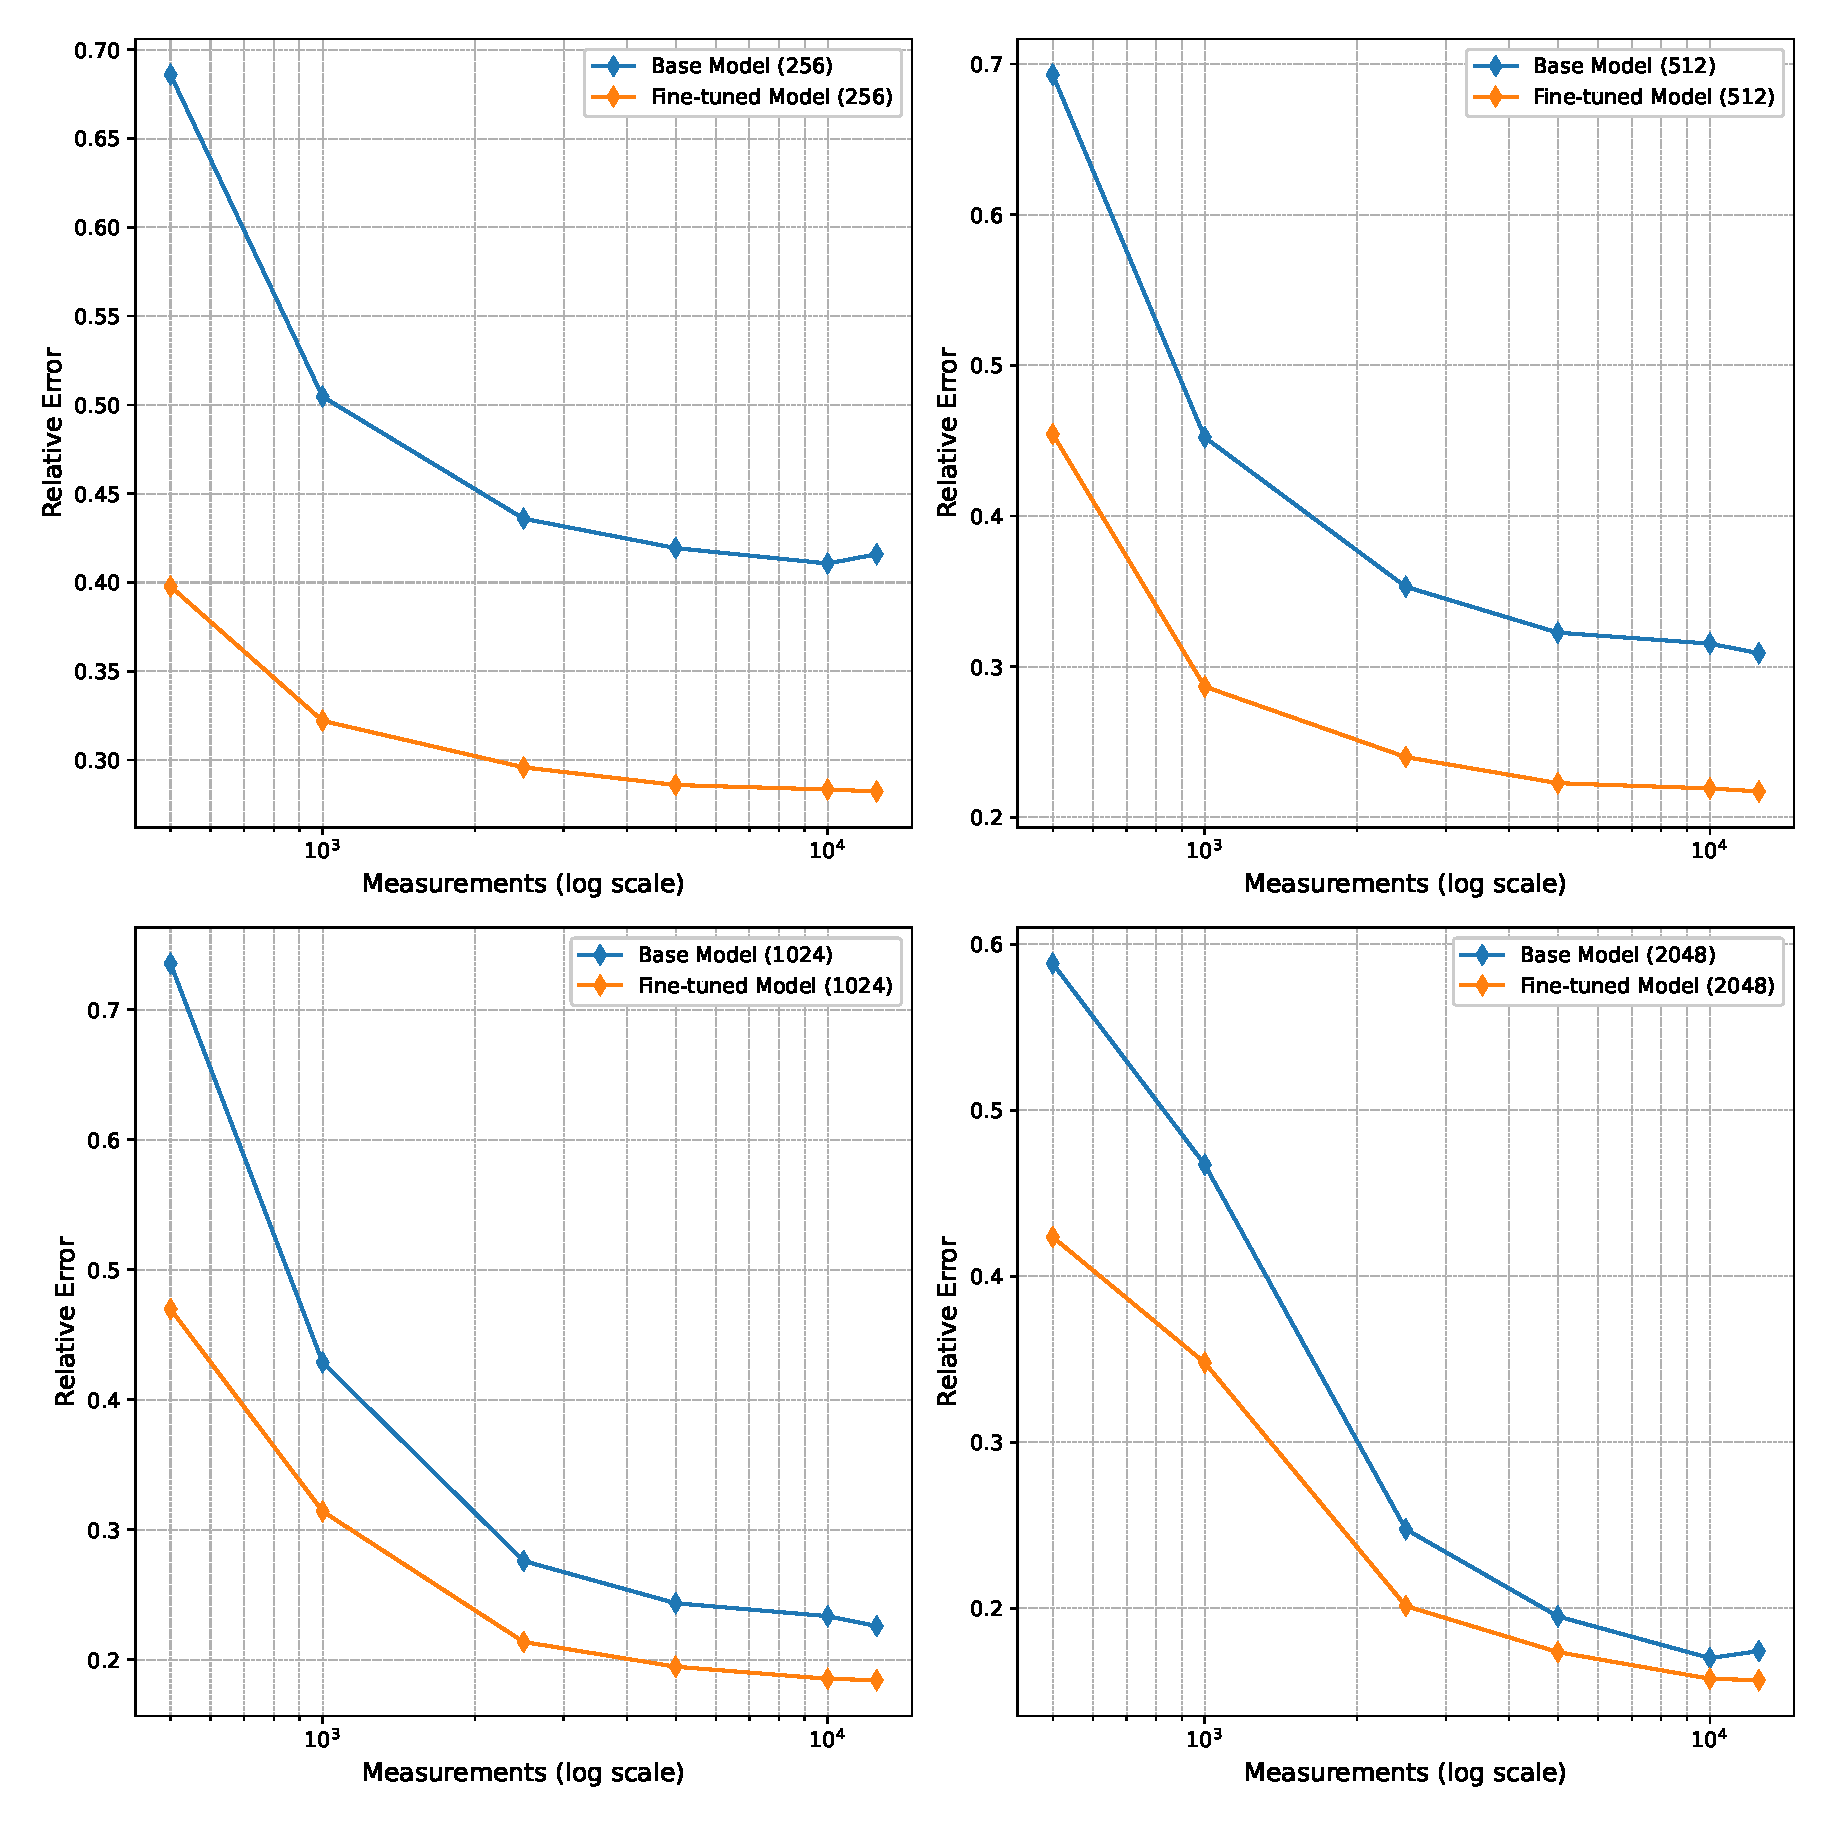
\includegraphics[width=\textwidth]{figures/06_results/fine_tuned_zuerich.eps}
%     \caption{Results for Fine-tuned Model Zurich}
% \end{figure}
% The other plots can be seen in the appendix.
% Overall, they follow the same trend.

\subsection{VAE vs Lasso}
\begin{figure}[h!]
    \centering
    \begin{subfigure}[b]{0.49\textwidth}
        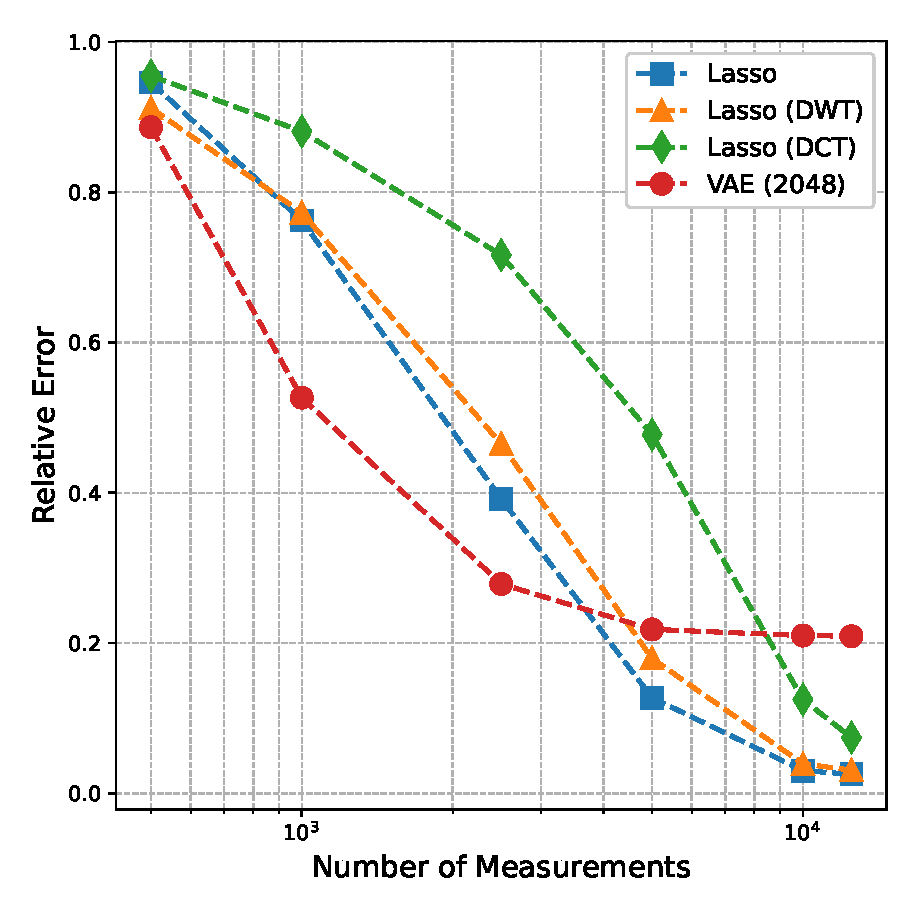
\includegraphics[width=\textwidth]{figures/06_results/vae_benchmark/vae_vs_lasso/vae_vs_lasso_relative_error.eps}
        \caption{Relative Error}
    \end{subfigure}
    \begin{subfigure}[b]{0.49\textwidth}
        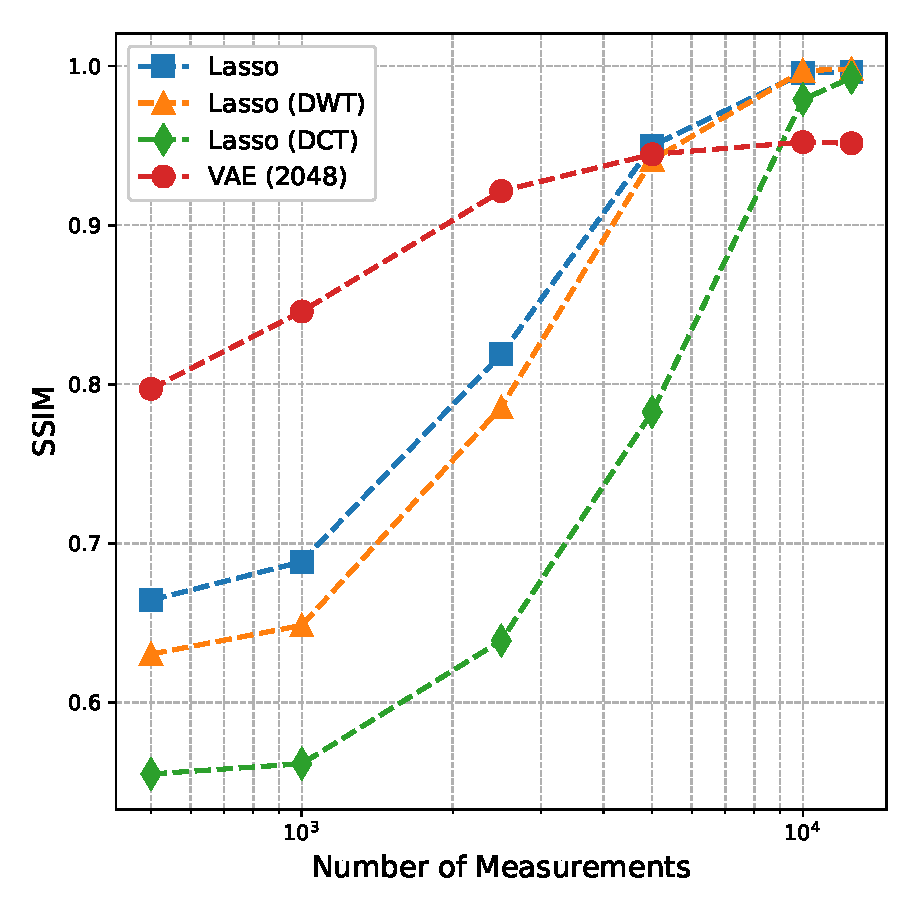
\includegraphics[width=\textwidth]{figures/06_results/vae_benchmark/vae_vs_lasso/vae_vs_lasso_ssim.eps}
        \caption{SSIM}
    \end{subfigure}
    \begin{subfigure}[b]{0.49\textwidth}
        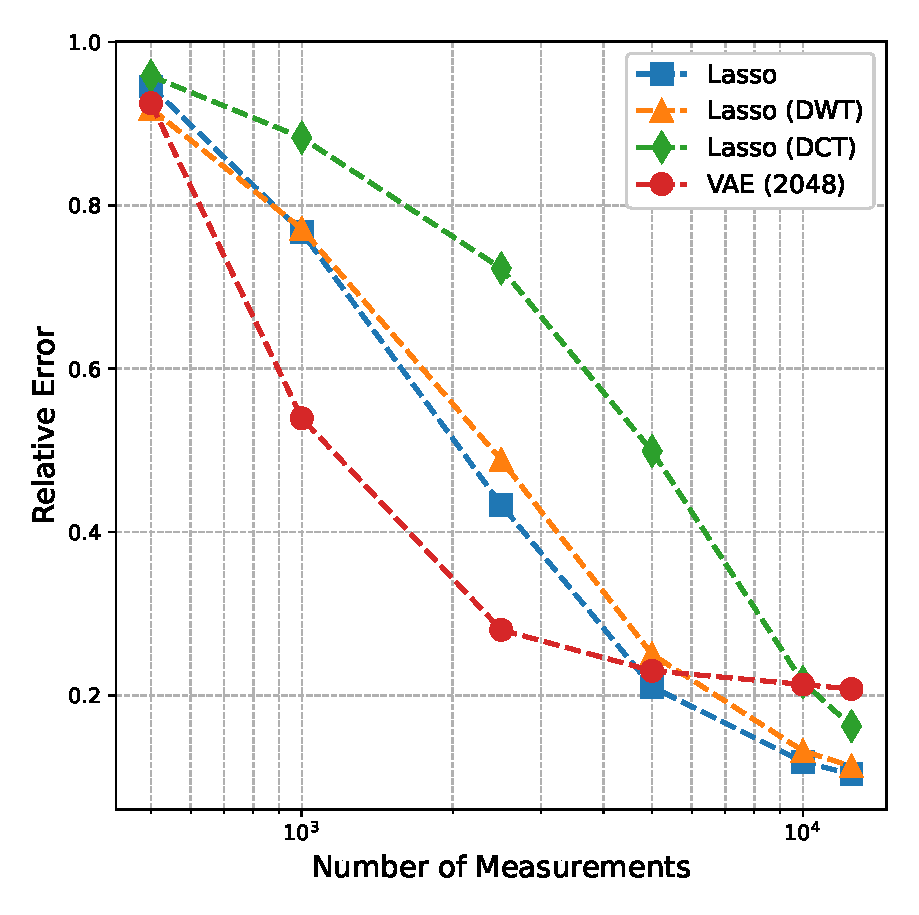
\includegraphics[width=\textwidth]{figures/06_results/vae_benchmark/vae_vs_lasso/vae_vs_lasso_relative_error_noisy.eps}
        \caption{Relative Error (20dB SNR)}
    \end{subfigure}
    \begin{subfigure}[b]{0.49\textwidth}
        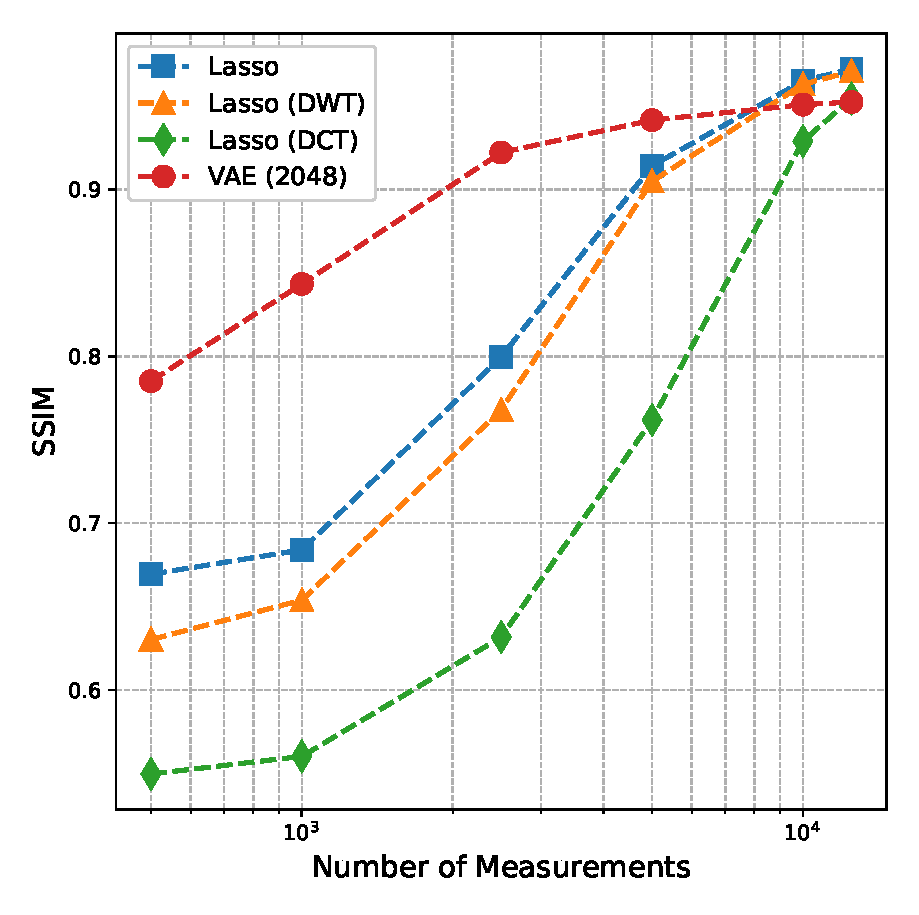
\includegraphics[width=\textwidth]{figures/06_results/vae_benchmark/vae_vs_lasso/vae_vs_lasso_ssim_noisy.eps}
        \caption{SSIM (20dB SNR)}
    \end{subfigure}
    \caption{VAE vs Lasso}
\end{figure}
Make a graph that keeps num measurements fixed and only varies the noise.

\section{Atmospheric Inversion}
\subsection{Over SNR}
The first run is an SNR plot.
For this run, the artifical footprints from Benjis paper are taken.
Jzst like in his paper, $3\%$ of unknowns measuement stations are used, i.e. 30.
Each measuement station takes $50$ measurements.
The signal to noise ratio is altered.
For each SNR, 3 problems are created to get better sampling.
\begin{figure}
    \centering
    \begin{subfigure}[b]{0.49\textwidth}
        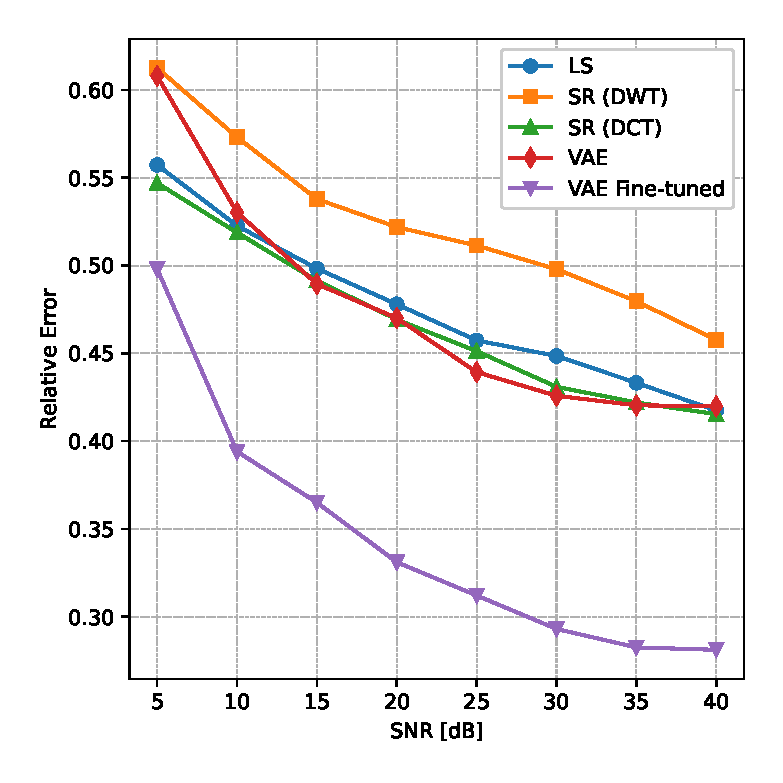
\includegraphics[width=\textwidth]{figures/06_results/snr_plots/munich_relative_error.eps}
        \caption{Relative Error}
    \end{subfigure}
    \begin{subfigure}[b]{0.49\textwidth}
        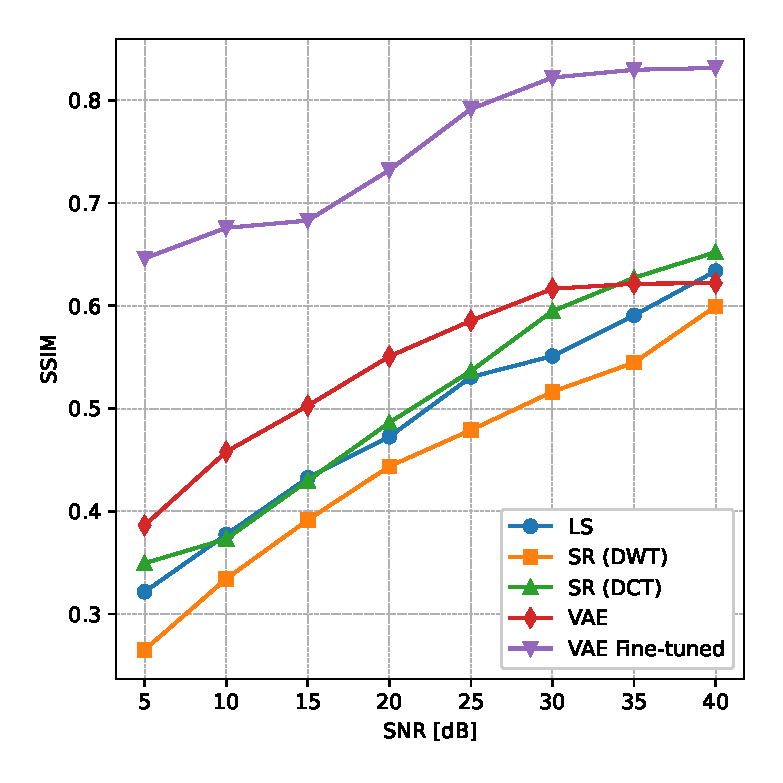
\includegraphics[width=\textwidth]{figures/06_results/snr_plots/munich_ssim.eps}
        \caption{SSIM}
    \end{subfigure}
    \caption{Results for Munich}
\end{figure}

\begin{figure}
    \centering
    \begin{subfigure}[b]{0.49\textwidth}
        \includegraphics[width=\textwidth]{figures/06_results/snr_plots/zürich_relative_error.eps}
        \caption{Relative Error}
    \end{subfigure}
    \begin{subfigure}[b]{0.49\textwidth}
        \includegraphics[width=\textwidth]{figures/06_results/snr_plots/zürich_ssim.eps}
        \caption{SSIM}
    \end{subfigure}
    \caption{Results for Zurich}
\end{figure}

\begin{figure}
    \centering
    \begin{subfigure}[b]{0.49\textwidth}
        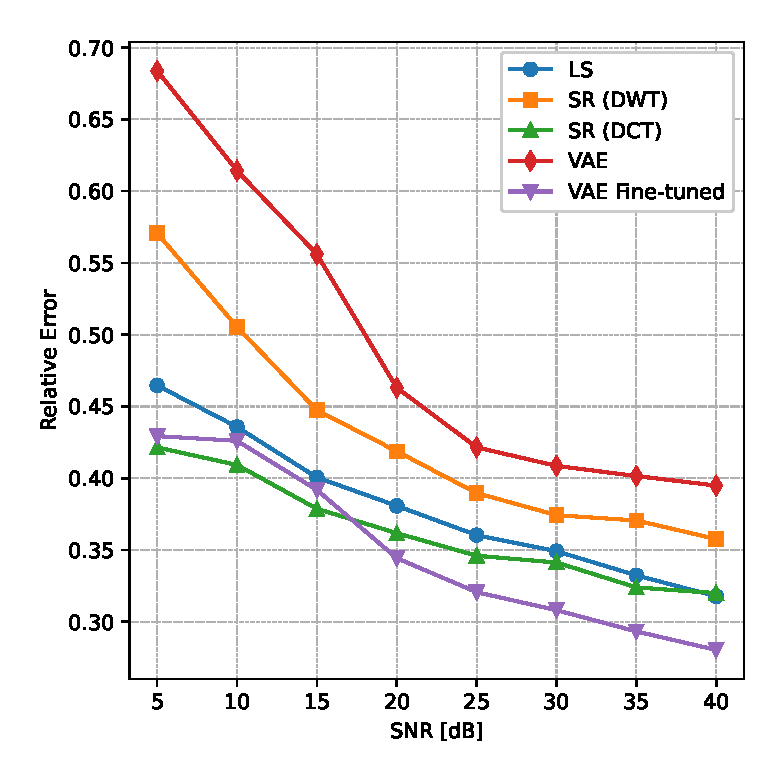
\includegraphics[width=\textwidth]{figures/06_results/snr_plots/paris_relative_error.eps}
        \caption{Relative Error}
    \end{subfigure}
    \begin{subfigure}[b]{0.49\textwidth}
        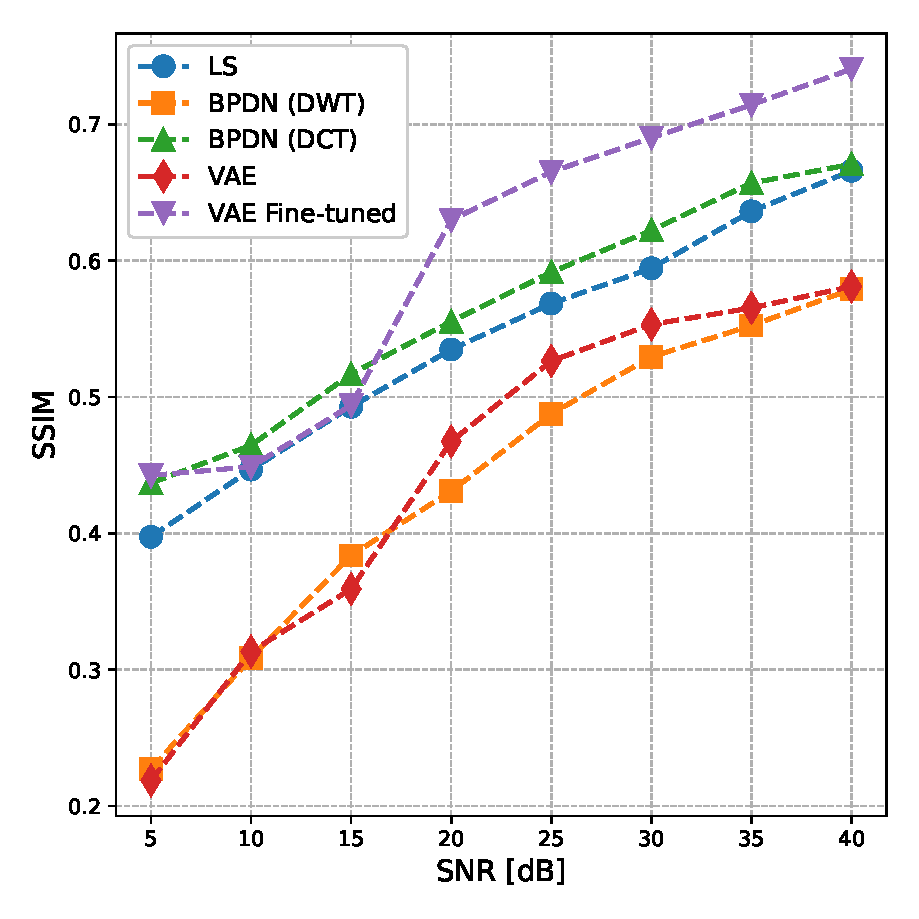
\includegraphics[width=\textwidth]{figures/06_results/snr_plots/paris_ssim.eps}
        \caption{SSIM}
    \end{subfigure}
    \caption{Results for Paris}
\end{figure}
Make a plot that has x axis snr and y axis relative error just like in Benjis plot.
Do this for the 3 cities.

\subsection{Example Munich}
The second run is an example to qualitatively assess the performance.
The situation is very favorable with a low to moderate SNR of 20dB.
The chosen city is Munich.
The example run was done with 13 measurement stations.
Each measurement station takes 50 measurements.
This results in 750 measurements.
The guassian plume simulation was run for a predefined wind field.
This wind field covers ~180 degrees.
\begin{figure}
    \centering
    \begin{subfigure}[b]{0.32\textwidth}
        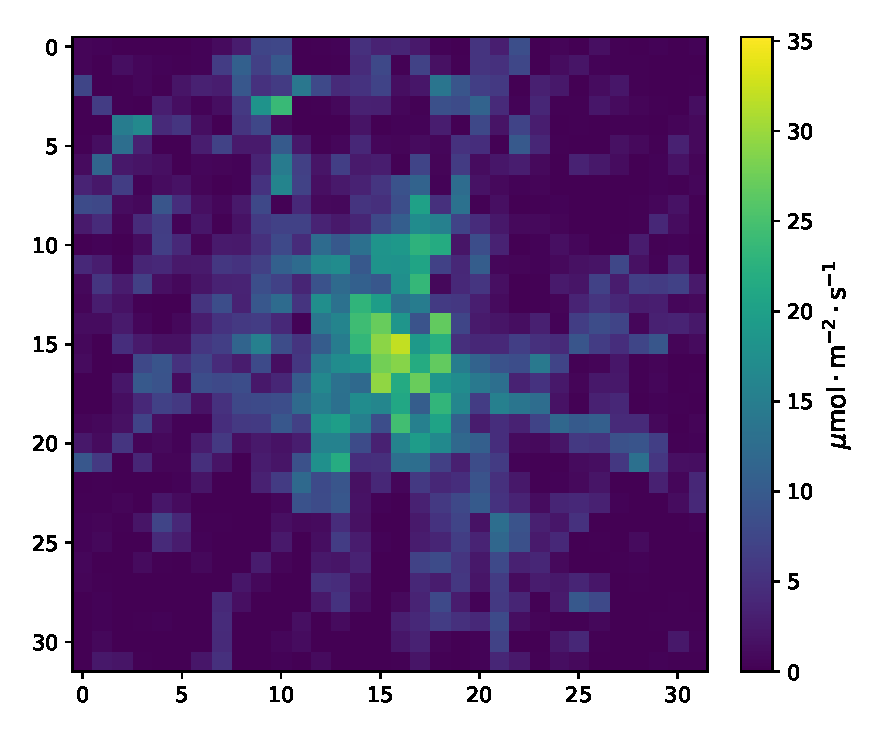
\includegraphics[width=\textwidth]{figures/06_results/gaussian_plume_example/munich/target.eps}
        \caption{Target Emissions}
    \end{subfigure}
    \begin{subfigure}[b]{0.32\textwidth}
        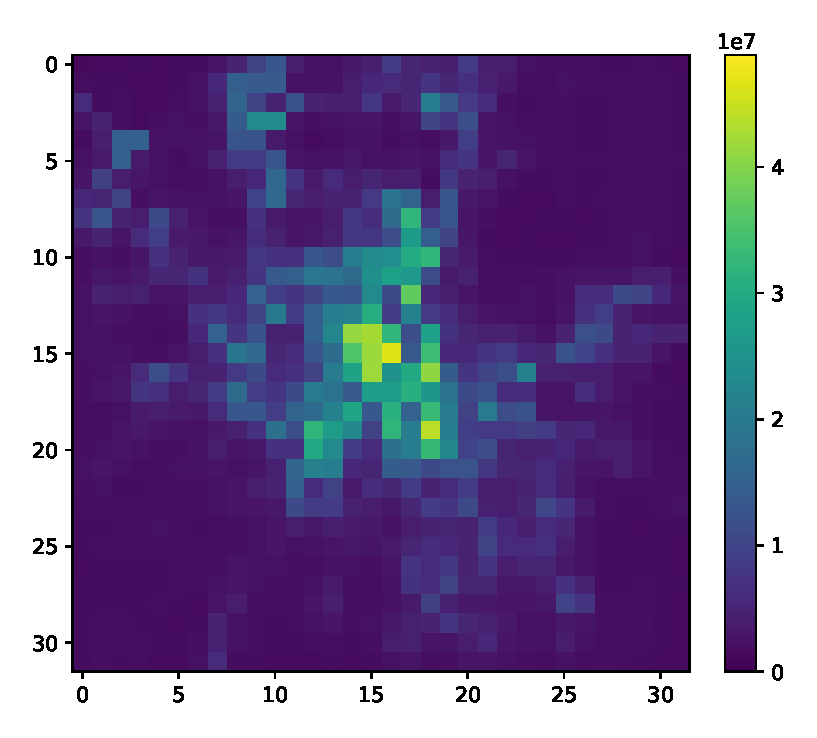
\includegraphics[width=\textwidth]{figures/06_results/gaussian_plume_example/munich/gen_2048_fine_tuned_20_db.eps}
        \caption{VAE (2048) Fine-tuned}
    \end{subfigure}
    \begin{subfigure}[b]{0.32\textwidth}
        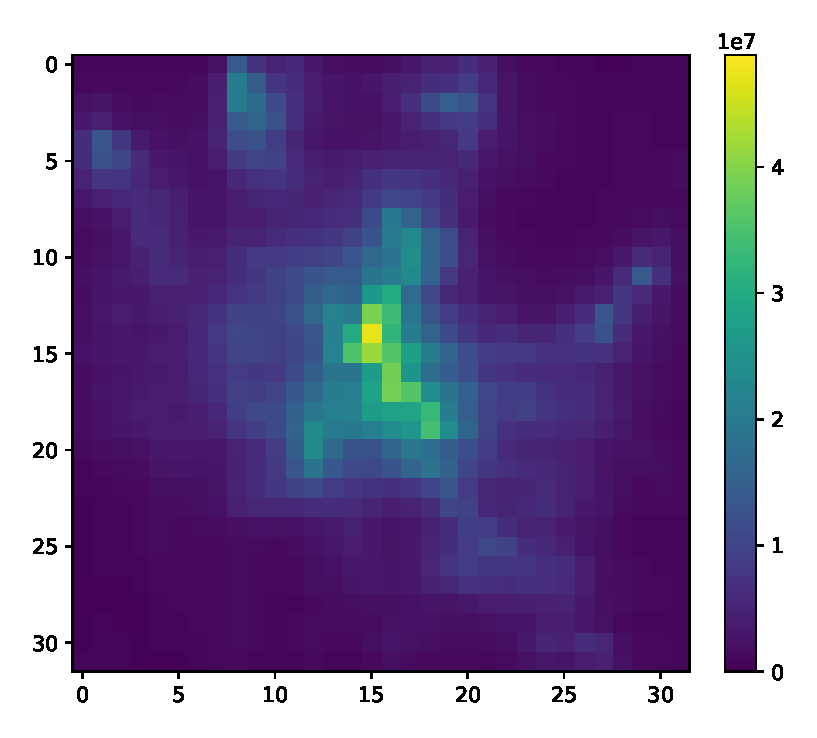
\includegraphics[width=\textwidth]{figures/06_results/gaussian_plume_example/munich/gen_2048_20_db.eps}
        \caption{VAE (2048)}
    \end{subfigure}
    \begin{subfigure}[b]{0.32\textwidth}
        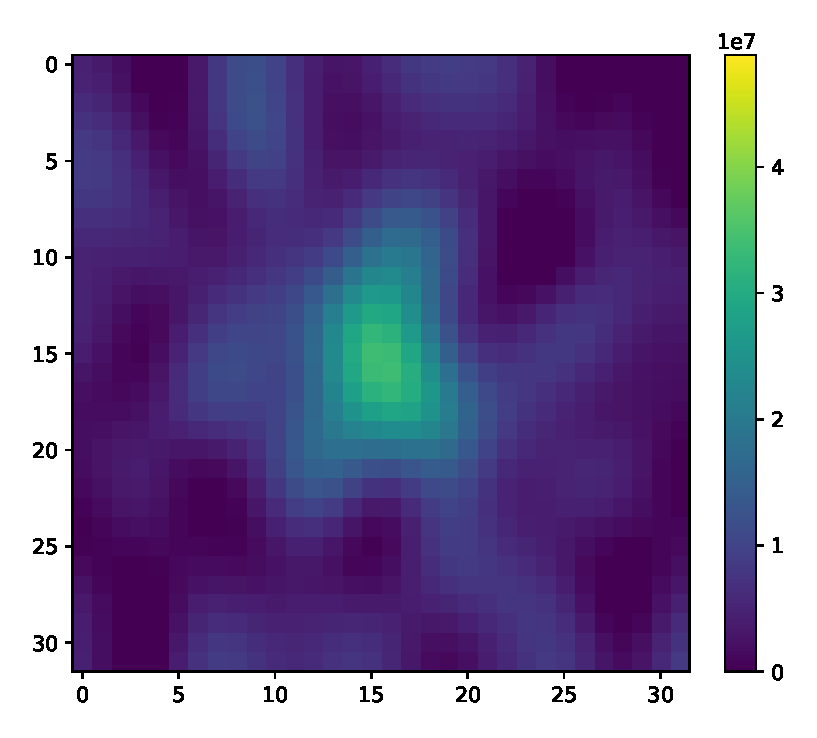
\includegraphics[width=\textwidth]{figures/06_results/gaussian_plume_example/munich/bp_dct_snr_20_db.eps}
        \caption{SR (DCT)}
    \end{subfigure}    
    \begin{subfigure}[b]{0.32\textwidth}
        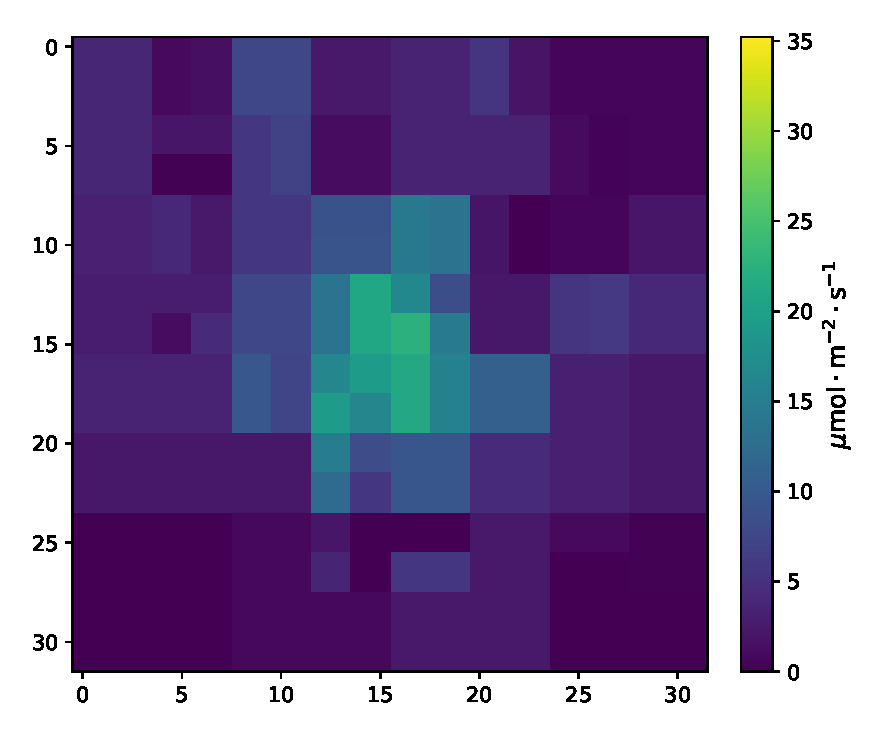
\includegraphics[width=\textwidth]{figures/06_results/gaussian_plume_example/munich/bp_dwt_snr_20_db.eps}
        \caption{SR (DWT)}
    \end{subfigure}
    \begin{subfigure}[b]{0.32\textwidth}
        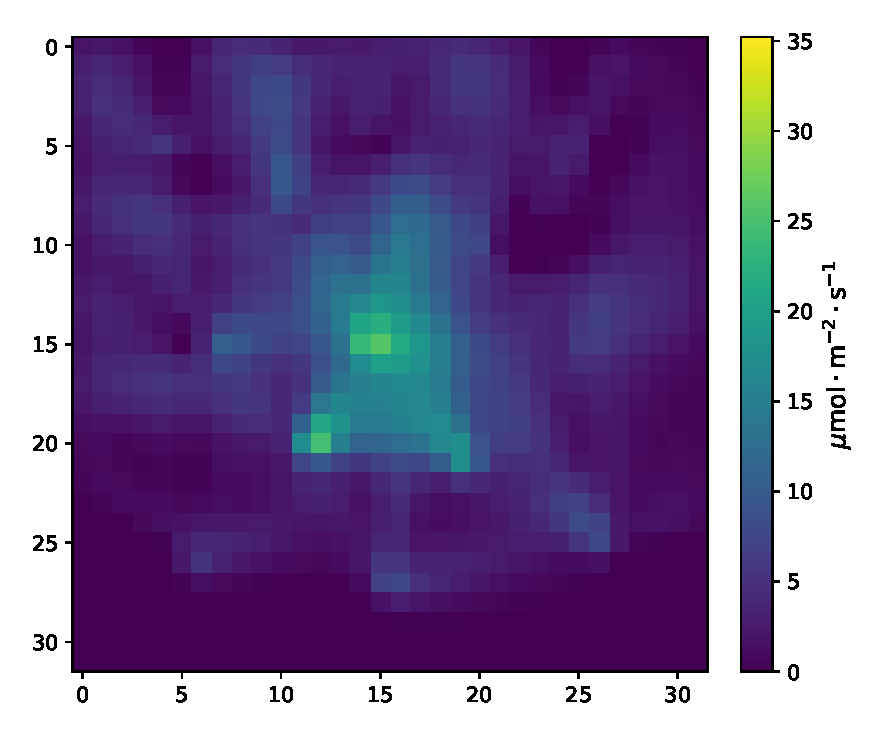
\includegraphics[width=\textwidth]{figures/06_results/gaussian_plume_example/munich/least_squares_snr_20_db.eps}
        \caption{LS}
    \end{subfigure}
    \caption{Example Run for Munich}
\end{figure}
The results are reported in the following table.
This also includes the other models that performed worse than the 2048 one.
\begin{table}[h]
    \centering
    \begin{tabular}{|l|c|c|}
        \hline
        \textbf{Solver} & \textbf{Relative Error} & \textbf{SSIM} \\
        \hline
        \hline
        VAE (256) & 54.880\% & 0.426 \\
        VAE (512) & 50.999\% & 0.499 \\
        VAE (1024) & 48.941\% & 0.493 \\
        VAE (2048) & 46.139\% & 0.520 \\
        \hline
        VAE (256) Fine-tuned & 46.333\% & 0.585 \\
        VAE (512) Fine-tuned & 35.974\% & 0.710 \\
        VAE (1024) Fine-tuned & 37.609\% & 0.739 \\
        \textbf{VAE (2048) Fine-tuned} & \textbf{32.833\%} & \textbf{0.751} \\
        \hline
        SR (DWT) & 51.102\% & 0.445 \\
        SR (DCT) & 47.767\% & 0.514 \\
        \hline
        LS & 49.767\% & 0.449 \\
        \hline
    \end{tabular}
    \caption{Relative Error and SSIM for Different Solvers}
    \label{tab:solvers}
\end{table}
TODO: add sum of sensitivities for this example.

% !TeX root = ../main.tex
% Add the above to each chapter to make compiling the PDF easier in some editors.

\chapter{Discussion}\label{chapter:discussion}

\section{Model}
The model is far from ideal.
By using MCMC, it was obvious that the latent variable could not be modeled as Gaussian.
By investigating the latent variable z it is obvious that the latent space does not follow a perfect Gaussian distribution.
We suspect that this has to do with the lack of distinct training samples.
Time sclaing does not fundamentally change the training sample.
Thus, fundamentally only n cities are contained in the training data.
We suspect that by gathering more training data, the model is able to capture the shape of the city emissions better.
Then, one could try to use algorithms such as MCMC.

This is also supported by the fact that a regularization factor \gls{gamma} of 0 works the best.

\section{Future Applciation}
This thesis presents the idea of using machine learning based solving of inverse problems with a technique from 2017.
The field of ML based inverse problems has made significant progress in the last year with research progress in generative AI.
This thesis only shows that such techniques are applicable to the problem of reconstructing emitters from measurements.
Thus, thie thesis opens the gates to exploring more of these approaches and apply state of the art techniques.

\section{To fill}
\begin{itemize}
    \item Uncertainty assessment possible with MCMC as MCMC outputs mean and variance for each pixel (citation needed)
\end{itemize}

% TODO: add more chapters here

\appendix{}

\microtypesetup{protrusion=false}

%\addchap{Abbreviations}
%\begin{acronym}
%\itemsep-.25\baselineskip
%\acro{TUM}[TUM]{Technical University of Munich}
% TODO: add acronyms
%\end{acronym}

\listoffigures{}
\listoftables{}
\microtypesetup{protrusion=true}
\printbibliography{}

\end{document}
